
\documentclass[a4paper,11pt,twoside,DIV10,english,numbers=noendperiod]{scrbook}
\usepackage[a4paper,left=3.5cm,right=2.5cm,bottom=3.5cm,top=3cm]{geometry}
%{report}

% ~~~~~~~~~~~~~~~my packages~~~~~~~~~~~`
% Multiline comments
\usepackage{verbatim}
%\usepackage[llncsdoc]{llncsdoc}
\usepackage{makeidx}  % allows for indexgeneration

%\usepackage{fullpage}
\usepackage[english]{babel}
\usepackage{graphicx}
\usepackage{multirow}
\usepackage{rotating}
\usepackage[latin1]{inputenc}
\usepackage[numbers,square]{natbib}
\usepackage{scrhack}
%Kapitel�berschriften in Gro�buchstaben
\setkomafont{chapter}{\normalfont \scshape \Huge}
\setkomafont{section}{\normalfont \bfseries \LARGE}
\setkomafont{subsection}{\normalfont \bfseries \Large}
\setkomafont{subsubsection}{\normalfont \bfseries \large}
\setkomafont{paragraph}{\normalfont \bfseries \large}
%Pallanoid Schriftart verwenden
\usepackage{mathpazo}

%Auswahl der Schriftart erm�gliche, damit Titelpage in Times und Rest in Pazo
\usepackage[T1]{fontenc}
\newcommand{\changefont}[3]{
\fontfamily{#1} \fontseries{#2} \fontshape{#3} \selectfont}

\usepackage{scalefnt}
\usepackage{titlesec}
\usepackage{titletoc}
\titleformat{\chapter}[display]
{\mdseries\huge\scshape}
{	\filleft
	\begingroup
		\scalefont{3}
			{\bfseries{\thechapter}}
	\endgroup}
{0ex}
{%\titlerule
\vspace{1ex}%
\filright}
[\vspace{1ex}%
\titlerule]

% Leere Seite ohne Seitennummer, naechste Seite rechts
\newcommand{\blankpage}{
 \clearpage{\pagestyle{empty}\cleardoublepage}
}

% Keine einzelnen Zeilen beim Anfang eines Abschnitts (Schusterjungen)
\clubpenalty = 10000
% Keine einzelnen Zeilen am Ende eines Abschnitts (Hurenkinder)
\widowpenalty = 10000 \displaywidowpenalty = 10000

%\usepackage[pdftex]{graphicx,color}
\usepackage{amsmath,amssymb,subfigure}

% Zeilenabstand einstellen %
\renewcommand{\baselinestretch}{1.25}
%\usepackage{setspace}
%\onehalfspacing

% Floating-Umgebungen anpassen %
\renewcommand{\topfraction}{0.9}
\renewcommand{\bottomfraction}{0.8}

% Theorem-Umgebungen
\usepackage[amsmath,thmmarks]{ntheorem}

% Caption Packet
\usepackage[margin=0pt,font=small,labelfont=bf]{caption}

% URLs
\usepackage{url}

% Bibtex deutsch
%\usepackage{bibgerm}

%\usepackage{abstract}

% Algorithmen

\usepackage{float}
\usepackage[ pdftex, plainpages=false, pdfpagelabels, hypertexnames=true, linktocpage=true, bookmarksopen=true, bookmarksopenlevel=1] {hyperref}
\usepackage[chapter]{algorithm}
\usepackage{algorithmic}

\setcounter{equation}{0}
% Theorem-Optionen %
\theoremseparator{.}
\theoremstyle{change}
\newtheorem{theorem}{Theorem}[section]
\newtheorem{satz}[theorem]{Satz}
\newtheorem{lemma}[theorem]{Lemma}
\newtheorem{korollar}[theorem]{Korollar}
\newtheorem{proposition}[theorem]{Proposition}
% Ohne Numerierung
\theoremstyle{nonumberplain}
\renewtheorem{theorem*}{Theorem}
\renewtheorem{satz*}{Satz}
\renewtheorem{lemma*}{Lemma}
\renewtheorem{korollar*}{Korollar}
\renewtheorem{proposition*}{Proposition}
% Definitionen mit \upshape
\theorembodyfont{\upshape}
\theoremstyle{change}
\newtheorem{definition}[theorem]{Definition}
\theoremstyle{nonumberplain}
\renewtheorem{definition*}{Definition}
% Kursive Schrift
\theoremheaderfont{\itshape}
\newtheorem{notation}{Notation}
\newtheorem{konvention}{Konvention}
\newtheorem{bezeichnung}{Bezeichnung}
\theoremsymbol{\ensuremath{\Box}}
\newtheorem{beweis}{Beweis}
\theoremsymbol{}
\theoremstyle{change}
\theoremheaderfont{\bfseries}
\newtheorem{bemerkung}[theorem]{Bemerkung}
\newtheorem{beobachtung}[theorem]{Beobachtung}
\newtheorem{beispiel}[theorem]{Beispiel}
\newtheorem{problem}{Problem}
\theoremstyle{nonumberplain}
\renewtheorem{bemerkung*}{Bemerkung}
\renewtheorem{beispiel*}{Beispiel}
\renewtheorem{problem*}{Problem}

% Algorithmen anpassen %
\renewcommand{\algorithmicrequire}[1]{\textbf{Eingabe:}#1\\}
\renewcommand{\algorithmicensure}[1]{\textbf{Ausgabe:}#1\\}
\floatname{algorithm}{Algorithmus}
\renewcommand{\listalgorithmname}{Algorithmenverzeichnis}

%Silbentrennung
\hyphenation{De-zi-mal-trenn-zeichen In-stal-la-ti-ons-as-sis-tent Ist-Schwer-punkt-po-si-tion}

\newcommand{\modelica}[3]{\vspace*{.75cm}
													\begin{addmargin}[0.5cm]{0.5cm} 
														\begin{minipage}{\linewidth}
															\noindent\rule[1ex]{\textwidth}{1pt}\\
															\noindent{\textbf{#1}\hfill\footnotesize(\textit{Modelica}-Quelltext - Auszug aus \ref{#2} auf Seite \pageref{#2})\normalsize}\\
															\noindent\rule[1ex]{\textwidth}{1pt}														
															\begin{flushleft}
																\hangindent=0.5cm #3	\\
															\end{flushleft}															
															\noindent\rule[1ex]{\textwidth}{1pt}\\
														
														\end{minipage}
													\end{addmargin}
													%\vspace*{.75cm}
												 }

\begin{document}
%\raggedbottom
	%\frontmatter

	\setcounter{secnumdepth}{3}
	\setcounter{tocdepth}{3}

	%\pagestyle{headings}  % switches on printing of running heads
	\pagenumbering{roman}
	
	%Schriftart f�r Titelseite auf TIMES
	\changefont{ptm}{m}{n}
	
	
\begin{titlepage}

 \sffamily

 \vspace*{-2cm}

 \begin{minipage}{0.48\linewidth}
  \includegraphics[width=1.0\textwidth]{Bilder/tud_logo_rgb}
 \end{minipage}
 
 \vspace*{5.7cm}
 %\begin{center}
 % \noindent{
 %\begin{minipage}{0.55\linewidth}
%	\hrulefill
 % \vspace{2.0cm}
% \end{minipage}}
 \hfil
 %\begin{minipage}{0.4\linewidth}
  % empty
 %\end{minipage}
 %\begin{minipage}{0.15\linewidth}
  % empty
 %\end{minipage}
 \hfil
 \begin{minipage}{0.7\linewidth}
  \begin{center}
    \Huge\textbf{Master Thesis}
  \end{center}
  \begin{center}
    \huge{Estimation of Underactuated Degrees of Freedom(DOF's) in Humanoid Robots}\\[3ex]
  \end{center}
  \vspace{0.75cm}
  \begin{center}
    \large{Rajesh Rajendran}\\
 
 \normalsize{rajesh.rajendran@tu-dortmund.de}\\[2ex]
    \large{\today}
  \end{center}
 \end{minipage}
 \hfil
 \begin{minipage}{0.05\linewidth}
  % empty
 \end{minipage}
 \begin{minipage}{0.55\linewidth}
% \vspace{2.0cm}
%  \hrulefill
 \end{minipage}
% \end{center}
 %\vspace*{2cm}

 \vfill
 			\rmfamily
 			\changefont{ppl}{m}{n}
 			\begin{table} [H]
				\centering
				\normalsize
				\begin{tabular}{p{0.53\textwidth}p{0.41\textwidth}}
					Examiner: & \\
					Name of first examiner & Name of second examiner\\
			  	&\\	
			  	Abteilung Informationstechnik\newline Institut f\"{u}r Roboterforschung  & Lehrstuhl des Zweitgutachters\newline Fakult\"{a}t f\"{u}r Informatik\\

			  \end{tabular}
			 \end{table}
			 
				\rmfamily
 				\changefont{ppl}{m}{n}

 \end{titlepage}
 
    %Schriftart wieder zur\"{u}ck auf pazo
    \changefont{ppl}{m}{n}



    \blankpage
    \newpage
    \tableofcontents
    \cleardoublepage

    \pagenumbering{arabic}
    \parindent 0pt
    % Buchstaben in Formeln bzw. Gleichungen sollten
% in einer Arbeit durchweg die gleiche Bedeutung haben.
% Um das zu unterst�tzen, die Schreibarbeit zu verringern,
% und Umbennungen zu vereinfachen sollten alle Bezeichner
% zentral in einer Datei als Makro definiert werden.

% Abk�rzungen
\newcommand{\IRF}{Institut f�r Roboterforschung}

% Formelvariablen
\newcommand{\Ri}[2]{R^{#1}_{#2}} % Rotationsmatrix von Frame #2 zu Frame #1
\newcommand{\Rv}[2]{R_v\left(#1, #2\right)} % Rotationsmatrix um beliebige Achse #1 bei Winkel #1

%    % Diese Datei dient als Testseite für Befehle oder Formeln. 
% Alle hier eingegebenen können direkt am Anfang der Arbeit betrachtet werden.

    %%%%%%%%%%%
    % Kapitel %
    %%%%%%%%%%%

    \chapter{Introduction}
\label{sec:einleitung}
The field of \emph{Robotics} have seen a tremendous development since the introduction of the term by \emph{Isaac Asimov} in 1940s. The fundamental components of robotic systems are mechanical structure, actuators, sensors and controller. Robotic system ranges from simple \emph{Cartesian manipulator} to the complex \emph{Humanoids}. \emph{Industrial robots} are robots that are used in applications such as palletizing, material loading and unloading, part sorting, packaging etc. These robots usually operate in the structured environment whose geometrical or physical characteristics are known in priori. They are pre programmed to execute the set of tasks. These robots have largely aided the automation of manufacturing processes in the industries. \emph{Mobile robots} that are used in the environments where human beings can hardly survive or be exposed to unsustainable risks are called \emph{Field robots}. \emph{Field robots} normally operate in the unstructured environments, where the geometry or physical characteristics are not know in priori. Mars rover \emph{Curiosity} is one such example. Locomotion in these robots are achieved either by wheels or by mechanical legs. Operating in the unknown environments and dynamic balancing of mechanical structure demands advanced control schemes for \emph{Field robots}.
\begin{comment}
a) structural improvement is limited
b) actuator is also limited
c) need for dexterous manipulation
c) Evolution in control strategy.
e) Model based controls.
d) limited sensors available.
f) need for filters
Chapter 2 : Discuss about walking 
Chapter 3 : State Estimation and Kalman Filtering
Chapter 4 : Results
 Even \emph{mobile robots} had some serious limitations in their deployability. For normal functioning these robots needed a flat surface which would be suitable for their smooth navigation and they do not have flexibility like human beings. For example, navigating through stairs is not possible with \emph{mobile robots}. These limitations ultimately encouraged the idea of having robots which have similar structural properties like humans, as it could be easily deployed in the human environment. This lead to the idea of Humanoid robots. Since then, research in this field have gained its importance. \emph{Toro} is the humanoid developed by DLR shown in Figure \ref{fig:toro}. \emph{Toro} is first built as a bipedal walker, which could execute human-like walking gait.
\begin{figure}[t]
  \centering
  \includegraphics[width=0.5\textwidth]{Bilder/Abbildung.pdf}
  %\caption{Eine Beispiel-Abbildung \cite{testref}.}
  \caption{Eine Beispiel-Abbildung.}
  \label{fig:bsp}
\end{figure}
\end{comment}
\section{Motivation}
\begin{itemize}
\item \textbf{Justify why is it important to solve this problem ?}
\end{itemize}

\section{Problem Statement}
    The focus of this thesis is estimation of underactuated degrees of freedom of a humanoid robot.  Degrees of freedom of a robot is the number of joints present in the robot \citep{mur94}. In contrast to fixed base manipulators where the degrees of freedom is equal to number of joints in robot, the degrees of freedom of a humanoid robot is equal to sum of number of joints and degrees of freedom of a single rigid body. The underactuated degrees of freedom of a humanoid robot are the degrees of freedom of a  rigid body.  A rigid body in three dimensional space can exhibit translational motion along \textbf{X,Y,Z} axes and rotational motion around these axes namely \emph{ roll, pitch ,yaw} as shown in Figure \ref{fig:rbody} in Chapter \ref{ch:multi_mdl}. The underactuated degrees of freedom are associated with a coordinate frame attached to the robot's body. In \emph{Toro} the coordinate frame is attached to the hip or base. Base connects the upper body and lower body of \emph{Toro}. As a result the state estimation problem involves estimation of motion parameters of the base namely position and velocity.

 \paragraph{Underactated degrees of freedom:}
    The underactuated degrees of freeedom means that the degrees of freedom are unactuated or not controlled. These degrees of freedom are free to move in space. For example in a two dimension space any object has 3 degrees of freedom, two translational degrees of freedom and one rotational degree of freedom. But when the object is constrained to its environment the number of degrees of freedom is less.
    \begin{figure}[H]
    \begin{center}
    \includegraphics[trim = 0mm 130mm 0mm 20mm, scale = 0.75 ]{Bilder/dof2d.pdf}
    \caption{ Degrees of freedom of two dimensional object}
    \label{fig:dof_2d}
    \end{center}
    \end{figure}
    Figure \ref{fig:dof_2d} show how an object loses its degrees of freedom when it is constrained in 2 dimension space. In Figure \ref{fig:dof_2d} a) represents the unconstrained rectangular object free to move in space, b) represents the rectangular object constrained to move only along x axis and c) represents fully constrained rectangular object. 
    
   The humanoid robots opreates in three dimensional space. When it is freely suspended(it is floating in air) it has six free degrees of freedom. But when it is constrained to its environment, the number of degrees of feedom decreses. In this thesis we aim to estimate the motion of these degrees of freedom of a humanoid robot with respect to a frame of refrence.   
\subparagraph{Illustartion:}    
     \begin{figure}[h]
	    \centering
    	\includegraphics[scale=0.75]{Bilder/robot_flatfloor}
	    \caption{Humanoid robot standing on flat surface}	
	    \label{fig:flat_floor}
    \end{figure}
   Figure \ref{fig:flat_floor} shows a simplified two dimensional version of a humanoid robot standing on the flat surface. The position and orientation of the hip can be determined by computing the forward kinematics of the robot. Forward kinematics is a function of joint angles and it is given as,
    \begin{equation}
    \label{eq:fwkin_flat}
    H_{hip}^s = \text{fwdkin}(q_1,q_2,q_3,q_4),
    \end{equation}
    where $H_{hip}^s$ is the homogeneous transformation matrix position and orientation of the hip with respect to spatial frame. 
    \begin{figure}[h]
	    \centering
    	\includegraphics[scale=0.65]{Bilder/robot_slope}
	    \caption{Humanoid robot standing on a slope}	
	    \label{fig:slope}
    \end{figure}
    Figure \ref{fig:slope} shows a humanoid robot staning on the sloping surface. In this case the orientation computed by the forward kinematics function in Equation \ref{eq:fwkin_flat} will be wrong. As we can see in the Figure \ref{fig:slope} there is an additional angle $\alpha$ acting between the surface of the real ground and the slope. There is no direct measuremnt available for this underactuaed degree of freedom. Failure to estimate this angle may lead to  tilting over an edge which might cause the robot to fall on the ground. Estimating this angle will help to achive good balancing in the humanoid robot.

 \section{Methodolgy} 
    Kalman filter is an optimal state estimator for linear systems. The popular nonlinear extensions of Kalman filters used in practice are Extended Kalman filter(EKF) and Unscented Kalman filter(UKF) \citep{oli12}\citep{atk12}\citep{bloe12}. The estimation problem is solved in both versions of Kalman filter. The results are compared based on accuracy of estimates and simulation time. Chapter \ref{ch:st_est} gives brief introduction to state estimation and describes the Kalman filtering algorithm. EKF and UKF algorithms are presented in Chapter \ref{ch:st_est}.

    Two different models used for the purpose of state estimation. They are the multi body system model and the model of Inertial measurement unit(IMU). A multi body system is a modelling foramlism that is used to model the dynamic behaviour of a multi body system. \emph{Toro} is modelled as a multibody system. \emph{Toro} has 25 joints or 25 degrees of freedom. In addition to these 25 degrees of freedom there are 6 underactuad degrees of freedom. Altogether \emph{Toro} has 31 degrees of freedom. State estimation of the multi body system involves estimation of position and velocity of the degrees of freedom of the system. For example in \emph{Toro} has 31 degrees of freedom. The result of estimation problem will be 31 poitions and 31 velocities which leads to 62 states being estimated. Chapter \ref{ch:multi_mdl} deals with the modelling of multibody systems and its implementation in Kalman filtering algorithm. 
    
    A simplified model of IMU is discussed in Chapter \ref{ch:simp_mdl}. State estimation using this model involves estimating the position, orientation, translational velocity, accelerometer bias and gyroscope bias. The position, orientation estimated are the underactuated degrees of freedom and of \emph{Toro}. Translational velocity is the velocity of translationl motion of \emph{Toro}. The number of estimated states are 15. State estimation using this model is more simpler than the multi body system. It is practically implemented on \emph{Toro}.

    %\chapter{Grundlagen}
\label{sec:Grundlagen}

    \chapter{State Estimation}
State estimation is the principle of estimating the internal state of the system from the measurement of inputs and outputs of the system. In general knowledge of the internal state of the system will make the system easy to control. Figure \ref{fig:observer} shows the usage of state estimator in state feedback control loop.
\begin{figure}[h]
  \centering
  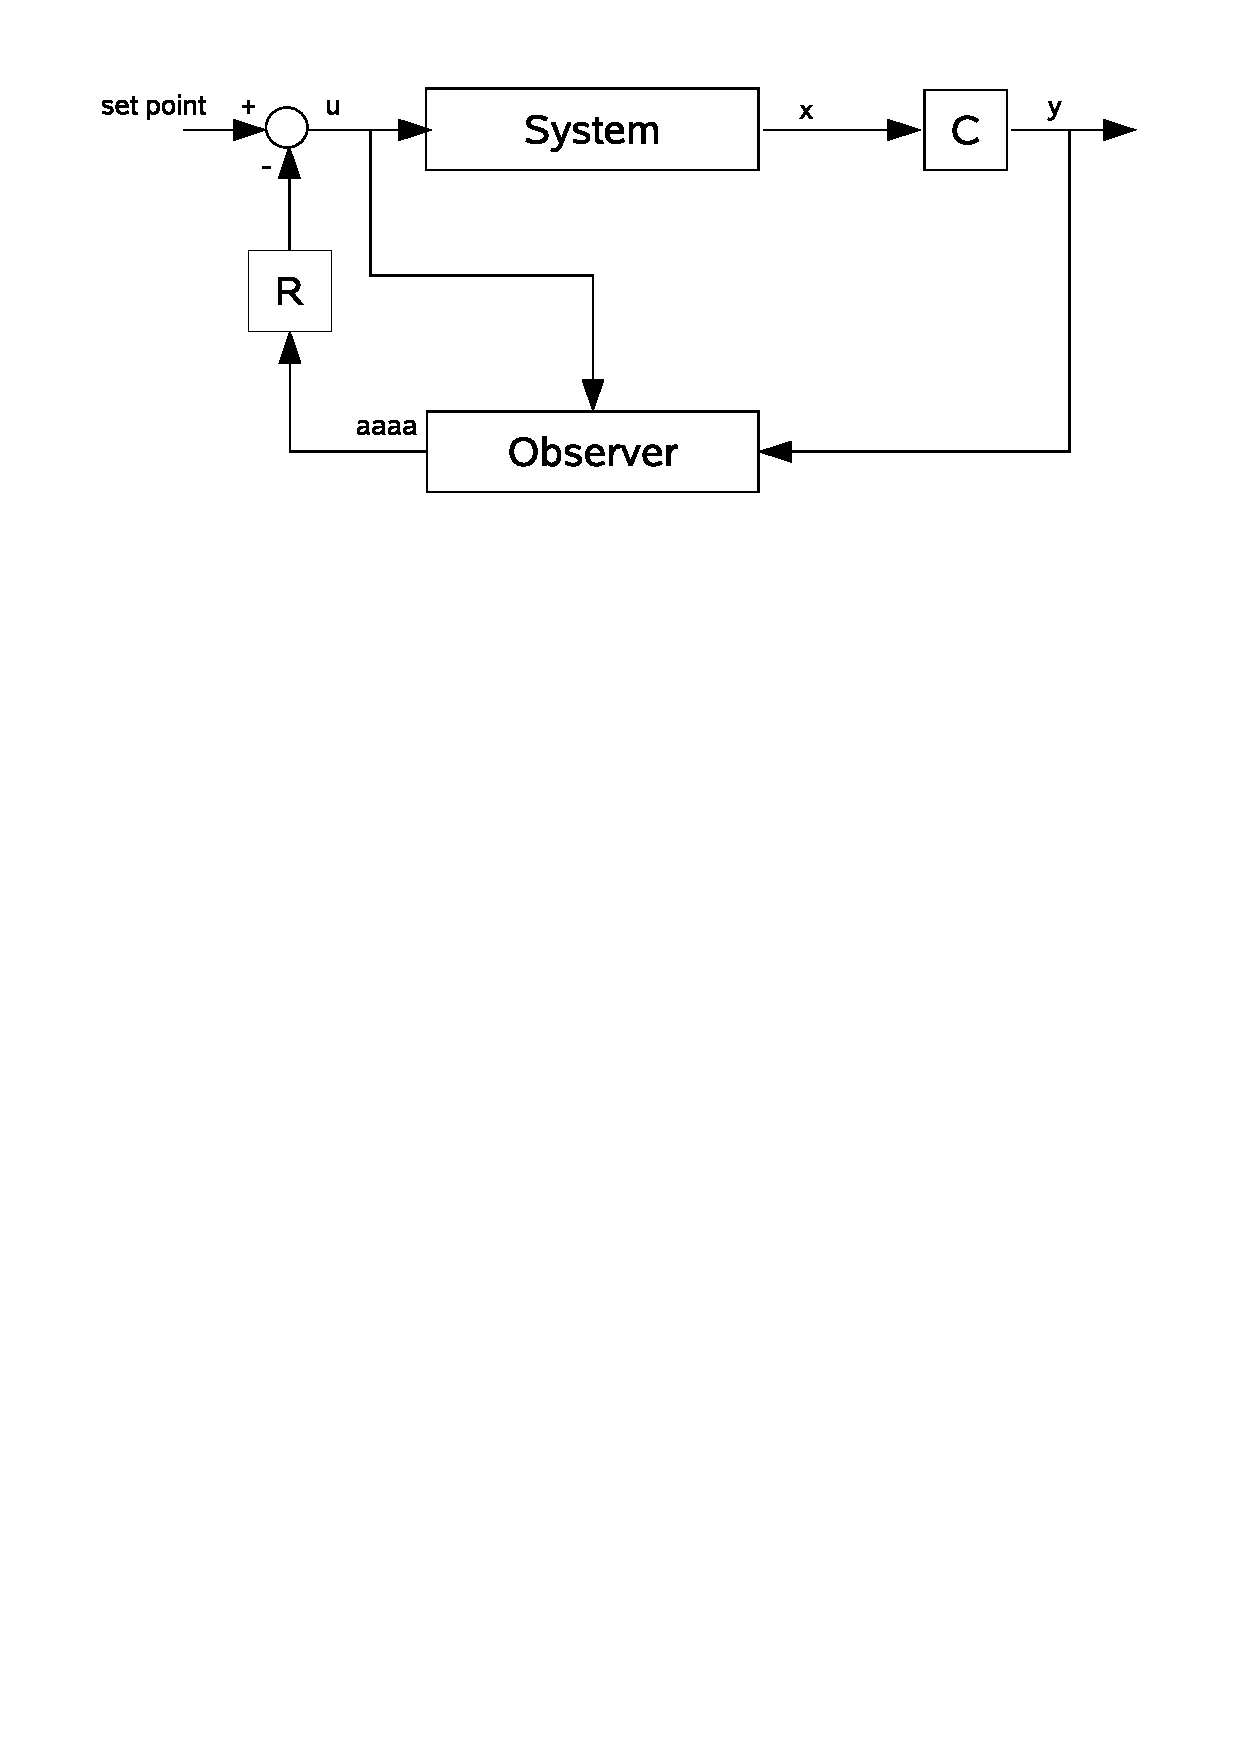
\includegraphics[trim = 10mm 200mm 20mm 20mm, clip,scale=0.80]{Bilder/system_observer.pdf}
  \caption{Structure of state feedback controller with state estimator}
  \label{fig:observer}
\end{figure}

A general nonlinear system in state space form,
\begin{equation}
\begin{split}
\label{eqn:nl_sys}
\dot{x}(t) &= f(x(t),u(t)) , x(t=0) = x_0 \\
y(t) &= g(x(t),u(t))
\end{split}
\end{equation}

In Equation \ref{eqn:nl_sys}, \emph{x(t)} represents the vector of internal states, \emph{u(t)} represents the vector of inputs and \emph{y(t)} represents the vector of outputs of the system. $x_0$ is the initial state of the system which is usually unknown. 
The state estimator is described by the system equation with additional correction term
\begin{equation}
\begin{split}
\label{eqn:est_sys}
\dot{\hat{x}}(t) &= f(\hat{x}(t),u(t)) + K(y(t)-\hat{y}(t)) , \hat{x}(t=0) = \hat{x}_0\\
\hat{y}(t) &= g(\hat{x}(t),u(t))
\end{split}
\end{equation}
$\hat{x}(t)$ is the state vector of estimator and \emph{K} is the gain matrix.  A state estimator should satisfy the following properties
\begin{itemize}
\item \textbf{Simulation property:} For the same initial condition $x(t_0) = \hat{x}_0$ of the estimator and the system to be observed, then it holds that $x(t) = \hat{x}(t) \forall t > 0 $.
\item \textbf{Convergence property:} If $x(t_0) \neq \hat{x}_0$, then $x(t) - \hat{x}(t)$ tends to zero as $ t \rightarrow \infty $
\end{itemize}

The different approaches for state estimator design differs in the calculation of gain matrix \emph{K} in Equation \ref{eqn:est_sys}.

\section{Kalman Filter}
Kalman filter is a statistical state estimation algorithm which gives the optimal estimate of internal state of the system from the noisy measurements. Kalman filter has widely used state estimator.
    \section{Kalman Filter}
Kalman filter is a statistical state estimation algorithm which estimates the internal state of the system from the noisy measurements. It was designed by Rudolph E. Kalman in 1960 for discrete time linear systems. It is basically a predictor-corrector type estimator that is optimal in the sense that it minimizes the estimated error covariance. Kalman filters provides good estimates in presence of modelling errors in system. Since the measurements occur and the states are estimated at discrete points of time, it is easily implementable in digital computers. Kalman filters are extensively used in the area of autonomous and guided navigation.

\subsection{Kalman gain}
A discrete time linear system affected by random noise is
\begin{equation}
    \begin{split}
        \label{eq:lin_ss}
        x_{k} &= Ax_{k-1} + Bu_k + w_{k-1}\\
        y_k &= Cx_k + v_k,
    \end{split}
\end{equation}
where the random variables $w_k$,$v_k$ represent the process and measurement noise. Both the random variables are assumed to be zero mean Gaussian white noises. Let $Q,R$ be the covariance of process and measurement noise. The error between the actual and predicted value of the state is \citep{gre01}
\begin{equation}\label{eq:kf_err}
e_k^ = x_k - \hat{x}_k,
\end{equation} 
where $x_k$ represents the true states of the system and $\hat x_k$ \footnote{ The estimated states are represented by hat symbol at the top, inorder to differentiate them from the true states of the system. For example $\hat x_k$ represents the estimated states} represents the estimated states.
The covariance of the error equation or the process covariance is 
\begin{equation}\label{eq:kf_P}
P_k^ = E[e_k {e_k}^T].
\end{equation} Kalman filter corrects its estimate based on the predicted state and measured output data by 
\begin{equation} \label{eq:kf_correct}
\hat{x_k} = \hat{x}_k + K(y_k - H\hat x_k).
\end{equation}
Kalman gain is computed by substituting Equation \ref{eq:kf_correct} in Equation \ref{eq:kf_err} to compute the $e_k^-$. Computed $e_k^-$ is substituted in Equation \ref{eq:kf_P} and the expected values are computed to find the error covariance $P_k^-$. Finally \emph{K} is computed by taking the derivative of trace of $P_k^-$ and equating it to zero $$ \dfdx{trace(P_k^-)}{K} = 0 $$ solving the above equation for \emph{K}. One form of \emph{K} that minimizes Equation \ref{eq:kf_correct}
\begin{equation} \label{eq:kf_gain}
 K_k = P_k^- C^T(C P_k^- C^T + R)^{-1}
    \end{equation}
From the Equation \ref{eq:kf_gain} as measurement covariance \emph{R} approaches zero, Kalman gain \emph{K} lays more trust on actual measurement $y_k$. On the other hand if $P_k^-$ approaches zero, predicted measurement $C\hat{x_k}^-$ is trusted more.

\subsection{Extended Kalman filter}
Most of the real world estimation scenarios are non linear in nature. Kalman filter algorithm  being a linear state estimation algorithm cannot be applied to the non linear systems. \emph{NASA Ames} devised a method to apply Kalman filter for non linear systems which is called the Extended Kalman filter(EKF) \citep{ekf85}. In EKF the non linear system is linearised by multivariate Taylor series expansion of the non linear function. 

The discrete time non linear system in state space representation is
\begin{equation}
\label{eq:nl_disc}
\begin{split}
x_{k} &= f(x_{k-1},u_k,w_{k-1})\\
y_k &= h(x_k,u_k,v_k),
\end{split}
\end{equation}
\emph{x,y} denotes the vector of system's state and output. \emph{w,v} represents the process and measurement covariance noise. The non linear funcion that relates the previous state to the present state is  $f(x_{k-1},u_k,w_{k-1})$ and $h(x_k,u_k,v_k$) is the non linear function that relates the output and state. 

In practice the individual values of noise $w_k$ and $v_k$ at each time step \emph{k} is not known. So one can compute the approximated state and measurement vector without them as 
\begin{equation}
\begin{split}
\label{eq:ekf_priori}
\hat{x}_k^- &= f(\hat{x}_{k-1},u_{k},0)\\
\hat{y}_k &= h(\hat{x}_k^-,u_{k},0),
\end{split}
\end{equation}
where $\hat{x}_k^-$\footnote{The priori state estimates are indicated by the $-$ sign in the superscript of the symbol. For example $\hat x_k^-$ represents the prori state estimate.} is the called the priori state estimate. The priori state estimate is used to compute the measurement $\hat{y}_k$ at time step \emph{k}. For the computation of Kalman gain $K$ in Equation \ref{eq:kf_gain}, $P_k$ and $C_k$  have to be computed. The state covariance matrix $P_k$ is $$P_k = A_k P_{k-1} A_k^T + W_k Q_{k-1} W_k^T. $$ 
    $A_k$ and $C_k$  are the Jacobian matrices that results by taking partial derivative of $\hat x_k^-$ and $\hat y_k$ in Equation \ref{eq:nl_disc} with respect to \emph{x}  at time instant \emph{k}. The $A_k$ and $C_k$ are the linear equivalent of state and measurement matrices of non linear system described in Equation \ref{eq:nl_disc}. $W_k$ and $V_k$ are the noise correlation matrix of process and measurements. They are computed by taking  Jacobian of $\hat x_k^-$  with respect to \emph{w} and and $\hat y_k$ with respect to \emph{v} in Equation \ref{eq:nl_disc}.
\begin{equation}
\begin{split}
A_k(i,j) &= \dfdx{f_i}{x_j}(\hat{x}_{k-1},u_k,w_{k-1})\\
C_k(i,j) &= \dfdx{h_i}{x_j}(\hat{x}_k^-,u_k,v_k)\\
W_k(i,j) &= \dfdx{f_i}{w_j}(\hat{x}_{k-1},u_k,w_{k-1})\\
V_k(i,j) &= \dfdx{h_i}{v_j}(\hat{x}_k^-,u_k,v_k)\\
\end{split}
\end{equation}
The priori state estimates in Equation \ref{eq:ekf_priori} are corrected according to Equation \ref{eq:kf_correct}. The corrected estimate is called the posteriori state estimate. It is given by
\begin{equation}
    \hat{x}_k = \hat{x}_k^- + K_k(y_k-h(\hat{x}_k^-,u_k,0)).
\end{equation}
The correction for the process covariance matrix is given by
\begin{equation}
P_k = (I- K_kC_k)P_k^-.
\end{equation}

\subsubsection{Algorithm}
\begin{figure}  
\tikzset{state/.style={ rectangle,rounded corners, draw=black, very thick, minimum height=2em, inner sep=2pt, text centered,}, }
\begin{tikzpicture}[->,>=stealth']
% Prediction or Time update
 \node[state,
      ] (predict) 
       {\begin{tabular}{c}
       \textbf{Time update:}\\
       \hrulefill\\
       $\begin{matrix}
       \hat{x}_k^- = f(\hat{x}_{k-1},u_k,0) \\
       \hfill \\
       P_k^- = A_k P_{k-1} A_k^T+ W_k Q_{k-1} W_k^T 
       \end{matrix}$
       \end{tabular}
       };
       % Correction or Measurement update
       \node[state,       % layout (defined above)
       text width=6.5cm,  % max text width
       right of=predict,    % Position is to the right of QUERY
       node distance=8.5cm,    % distance to QUERY
       anchor=center] (correct) 
       {\begin{tabular}{c}
       \textbf{Measurement upadate:}\\
       \hrulefill\\
       $\begin{matrix}
       K_k = P_k^-C^T(C_kP_k^-C_k^T + V_kR_kV_k^T)^{-1}\\
       \hfill \\
       \hat{x}_k = \hat{x}_k^- + K_k(y_k-h(\hat{x}_k^-,u_k,0))\\
       \hfill \\
       P_k = (I- K_kC_k)P_k^-
       \end{matrix}$
       \end{tabular}
       };
% draw the paths and and print some Text below/above the graph
\path (predict)     edge[bend left]  node[anchor=south,above]{$\hat x_k^-, P_k^-$} (correct)
(correct)       edge[bend left] node[anchor= north,below] {$\hat x_{k-1}, P_{k-1}$} (predict);
\end{tikzpicture}
\caption{Recursive formulation of EKF}
\label{fig:ekf_blk}
\end{figure}

    The recursive formulation of the discrete time EKF is shown in Figure \ref{fig:ekf_blk}.  For every time step \emph{k}, the time update stage projects the current state estimates ahed of time. The measurement update stage corrects the projected estimate. For the next time step $k+1$ the posteriori estimates are time step $k$ from measurement update sage is used to project the state and its error covariance estimates.

The algorithm for discrete time EKF can be given as two steps.
\begin{itemize}
    \item \textbf{Time update or Predict}
\begin{equation}
\label{eq:ekf_predict}
\begin{aligned}
&\text{Project the state}\\
&\hat{x}_k^- = f(\hat{x}_{k-1},u_k,0)\\
&\text{Project the error covarience}\\
&P_k^- = A_kP_{k-1}A_k^T + W_kQ_{k-1}W_k^T\\
\end{aligned}
\end{equation}
\item \textbf{Measurement Update or Correct}\\
\begin{equation}
\label{eq:ekf_correct}
\begin{split}
&\text{Compute Kalman gain}\\
&K_k = P_k^-C^T(C_kP_k^-C_k^T + V_kR_kV_k^T)^{-1}\\
&\text{Update the estimate with measurement }y_k\\
&\hat{x}_k = \hat{x}_k^- + K_k(y_k-h(\hat{x}_k^-,u_k,0))\\
&\text{Update the error covariance} \\
&P_k = (I- K_kC_k)P_k^-
\end{split}
\end{equation}
\end{itemize}

The EKF algorithm is applied for the multi body system model of \emph{Toro} in Chapter \ref{ch:multi_mdl} and for the simplified model of IMU in Chapter \ref{ch:simp_mdl}.

The continuous time EKF algorithm is given by \citep{gel74}
\begin{equation}
    \label{eq:ekf_con}
    \begin{split}
        \dot {\hat x} &= f(\hat x,u) + K ( y-h(\hat x))\\
        \dot P(t) &= A(t)P(t) + P(t)A(t)^T + Q - P(t)H(t)^TR^{-1}H(t)P(t)\\
        K(t) &= P(t)H(t)^TR^{-1},
    \end{split}
\end{equation}
where $$A(t) = \dfdx{f}{x}(\hat x(t), u(t)), \hspace{2cm} H(t) = \dfdx{h}{x} (\hat x(t), u(t))$$ are the Jacobians of the state and measurement equation. The continuous time EKF is applied for the inverted double pendulum system in Chapter \ref{ch:multi_mdl}.

\subsubsection{Tuning rules:}
\label{subsec:tune_ekf}
Tuning of the EKF involves setting the values of the noise covariance matrices $Q,R$. When the measurements $y$ are noisy then the emphasis is laid on the prediction model. In other words the prediction model is relied more. This is achived by setting the covariances $Q<R$. On the other hand if the estimated process is noisy due to unmodelled dynamics or model mismatch then the measurements are relied more. This is achived by setting $Q>R$.

The initial convergence of the filter depends upon the initial values of the estimator's state $\hat x_0$ and covariance $P_0$. If a states of the estimated system is not known at the beginning then the initial state covariance $P_0$ is set to very high value to achive the fast convergence to actual value.

\subsection{Unscented Kalman filter}
The unscented Kalman filter is a new class filter for nonlinear systems. It was first addressed by Julier et.al in 1997 \citep{jul97} as an alternative to EKF. This filter introduces unscented transformation(UT) to propogate mean and covariance information through non linear transformations.
%This leads to a differnt method to compute the error covairance matrix $P_k^-$.

\subsubsection{Unscented transform}
The basic idea behined the UT was founded on the intuition that it is easier to approximate a probability distribution than it is to approximate an arbitrary nonlinear function \citep{jul04}. A set of sigma points are chosen so that their mean and covariance are $\bar x$ and $\Sigma_x$. The sigma points are applied to a non linear function which in turn yeild set of transformed points. The statistics computed from the transformed points forms the estimate of nonlinearly transformed mean and covariance. This method is similar to the one used by particle filters. The main difference is this method uses determinisic way to choose the sigma points based on the specific properties. 

The set $S$ consists of vectors of length $2n+1$ of sigma points $x_i$ and weights associated with the mean and covariance $W_i^m, W_i^c $. It is given by \citep{sim07} 
\begin{equation} 
    \label{eq:ut_sigma}
    \begin{split}
    S &= \{i= 0,1,...,2n:x_i,W_i \} \\
    x_0 &= \bar x \\ 
    x_i &= \bar x + \left[ \sqrt{(n+\lambda)\Sigma_x} \right ]_i \hspace{2cm} i = 1, \cdots ,n \\
    x_i &= \bar x - \left[ \sqrt{(n+\lambda)\Sigma_x} \right ]_{i-n} \hspace{2cm} i = 1, \cdots ,n . 
    \end{split}
\end{equation}
The matrix square root of a positive definite matrix $\Sigma_x$ is computed using Cholesky factorisation. 

The weights associated to the sigma points are given by 
\begin{equation}
    \label{eq:ut_weights}
    \begin{split}
    W_0^m &= \frac{\lambda}{n+\lambda} \\
    W_0^c &= \frac{\lambda}{n+\lambda} + ( 1 - \alpha^2 + \beta)\\
    W_i^m &= \frac{1}{2(n+\lambda)} \hspace{2cm} i = 1, \cdots, 2n \\
    W_i^c &= \frac{1}{2(n+\lambda)} \hspace{2cm} i = 1, \cdots, 2n ,
    \end{split}
\end{equation} 
where $\lambda$ is a scaling parameter given by $$ \lambda = \alpha^2(n+\kappa)-n. $$ The parameters $\alpha,\beta,\kappa$ are the tuning parameters of the UKF.
%To obtain an unbiased estimate the weights $W_i$ must obey the condition $$ \sum \limits_{i=0}^n W_i = 1. $$
The sigma points $x_i$ are applied to the non linear function $$y= f(x).$$ The mean $\bar y$, covariance $\Sigma_y$ and cross covariance $\Sigma_{xy}$ of the resulting sigma points are $y_i$ are given by
\begin{equation}
    \label{eq:ut_mean_cov}
    \begin{split}
        \bar y &= \sum \limits_{i=0}^{2n} W_i^m y_i \\
        \Sigma_y &= \sum \limits_{i=0}^{2n} W_i^c [y_i - \bar y ] [ y_i - \bar y] ^T \\
        \Sigma_{xy} &= \sum \limits_{i=0}^{2n} W_i^c [x_i - \bar x ] [ y_i - \bar y] ^T .
    \end{split}
\end{equation}

The UKF have all the steps as in the Kalman Filter. The continuous time non linear system with additive white noises $v(t),w(t)$ is as follows \citep{sim07}:
\begin{equation}
    \label{eq:ukf_nlsys}
    \begin{split}
       \frac{dx}{dt} &= f(x(t),u(t),t) + W(t)w(t) \\
       y(t) &= h(x(t),u(t),t) + V(t)v(t),
    \end{split}
\end{equation} 
where $W(t),V(t)$ are arbitrary time varying matrices independent of $x(t)$ and $y(t)$. For sake of simplicity we assume the white noises $v(t),w(t)$  are uncorrelated, so the matrices $W(t),V(t)$ are assmed as identity matrices. The difference between UKF and EKF is in the method used for computation of the state covariance $P_k$. The state covariace of the priori state estimate $\hat x_k^-$ projected ahed of time is $$ P_k^- = \sum \limits_{i=0}^{2n} W_i^c [\hat x_{i,k}^- - \hat{\bar x}_k^-] [\hat x_{i,k}^- - \hat{\bar x}_k^-]^T + Q. $$
Similarly the covariance matrix $\Sigma_{\hat y_k}$ after projecting the priori estimates through the nonlinear function is $$ \Sigma_{\hat y} = \sum \limits_{i=0}^n W_i^c [\hat{y}_{k,i} - \hat{\bar y}_k ] [ \hat{y}_{k,i} - \hat{\bar y}_k] ^T+R.$$
The cross covariance matrix $\Sigma_{\hat x_k^-, \hat y_k}$ is $$ \Sigma_{\hat x_k^- \hat y_k} = \sum \limits_{i=0}^{2n} W_i^c [\hat x_{k,i}^- - \hat{\bar x}_k^- ] [ \hat y_{k,i} - \hat{\bar y}_k] ^T .$$
The Kalman gain $K_k$ is $$K_k = \Sigma_{\hat{\bar x}_k^- \hat y_k} \Sigma_{\hat y_k}^{-1}.$$
The state and covariance are updated according to the following equations:
$$  \begin{aligned}
    \hat{\bar{x}}_k &= \hat{\bar{x}}_k^- + K_k(y_k - \hat{\bar y}_k)\\
    P_k &= P_k^- - K_k \Sigma_{y,k} K_k^T.
    \end{aligned}
    $$
\subsubsection{Algorithm}
The UKF algorithm in matrix form is given in \citep{sim07}. The matrix from UKF is chosen as it is easy to implement in Matlab.
\begin{itemize}
    \item \textbf{Unscented transform}
    \begin{equation}
        \begin{split}
            X &= [ \bar x \hspace{5mm} \cdots \hspace{5mm} \bar x ]+ \sqrt c [ 0 \hspace{5mm} \sqrt \Sigma_x \hspace{5mm} - \sqrt \Sigma_x ]\\
            Y &= g(X) \\
            \bar y &= Y w_m\\
            \Sigma_y &= Y W Y^T \\
            \Sigma_{xy} &= X W Y^T,
        \end{split}
    \end{equation}
    where $X$ is the matrix of sigma points. $c=\alpha^2(n+\kappa)$, the vector $w_m$ and matrix $W$ are given by
    \begin{equation}
        \begin{split}
        w_m &= [W_m^0 \hspace{5mm} \cdots \hspace{5mm} W_m^{2n} ]\\
        W &= (I-[w_m \hspace{2mm} \cdots \hspace{2mm} w_m])diag(W_c^0 \hspace{2mm} \cdots \hspace{2mm} W_c^{2n}) (I-[w_m \hspace{2mm} \cdots \hspace{2mm} w_m])^T.
        \end{split}
    \end{equation} 
    
    \item \textbf{Time update:} Project the state mean state mean $\hat{\bar x}^-_k$ and covariance ${\bar P}^-_k$ ahed of time. The time update is perfomed by the following steps:
    \begin{itemize}
        \item \textbf{Sigma points:} Compute the sigma points from the positeriori state estimates from the previous time step.
        \begin{equation}
        X_{k-1} = [ \hat{\bar{x}}_k \hspace{5mm} \cdots \hspace{5mm} \hat{\bar{x}}_k]+ \sqrt c [ 0 \hspace{5mm} \sqrt{P_{k-1}} \hspace{5mm} - \sqrt{P_{k-1}} ]
        \end{equation}

        \item \textbf{Unscented transform:} Propogate the sigma points through the non linear state projection function and compute their statistics.
        \begin{equation}
        \begin{split}
            &\hat X_k = f(X_{k-1},u_k,k-1) \\
            &\text{Mean of the transformed points }\\
            &\hat{\bar x}^-_k = \hat X_k w_m \\
        \end{split}
        \end{equation}

        \item \textbf{Estimate projection:} Compute the state covariance matrix from the projected estimates.
        \begin{equation}
            \hat{\bar P}^-_k = \hat X_k W \hat X_k^T + Q_{k-1}
        \end{equation}

    \end{itemize}
        
    \item \textbf{Measurement update:} The updated state mean $\hat{\bar x}_k$ and covariance ${\bar P}_k$. The measurement update is performed in the follwoing steps:
    \begin{itemize}
        \item \textbf{Sigma points:} Compute the sigma points from priori state estimates.
        \begin{equation}
        X_k^- = [ \hat{\bar{x}}_k^- \hspace{5mm} \cdots \hspace{5mm} \hat{\bar{x}}_k^-]+ \sqrt c [ 0 \hspace{5mm} \sqrt{P_k^-} \hspace{5mm} - \sqrt{P_k^-} ]
        \end{equation}

        \item \textbf{Unscented transform:} Propogate the sigma points through the measurement function and compute their statistics.
        \begin{equation}
        \begin{split}
        &\hat Y_k = h(X_{k}^-,u_k,k) \\
        &\text{Mean of the transfromed points}\\
        &\hat{\bar y}_k = \hat Y_k w_m \\
        &\text{Covariance of the transfromed points}\\
        &\Sigma_{\hat y_k} = \hat Y_k W \hat Y_k^T + R_k \\
        &\text{Cross covariance of the transformed points}\\
        &\Sigma_{\hat x_k^- \hat y_k} = \hat X_k^- W \hat Y_k^T \\
        \end{split}
        \end{equation}

        \item \textbf{Estimate Correction:} Compute the kalman gain and update the priori estimates.
        \begin{equation}
        \begin{split}
        &\text{Compute Kalman gain}\\
        &K_k = \Sigma_{\hat{\bar x}_k^- \hat y_k} \Sigma_{\hat y_k}^{-1}\\
        &\text{Update the priori state estimates}\\
        &\hat{\bar{x}}_k = \hat{\bar{x}}_k^- + K_k(y_k - \hat{\bar y}_k)\\
        &P_k = P_k^- - K_k \Sigma_{y,k} K_k^T
        \end{split}
        \end{equation}
    \end{itemize}
\end{itemize}
\begin{figure}  
% We need layers to draw the block diagram
\pgfdeclarelayer{background}
\pgfdeclarelayer{foreground}
\pgfsetlayers{background,main,foreground}

% Define a few styles and constants
\tikzstyle{sensor}=[draw, fill=blue!20, text width=5em, 
    text centered, minimum height=2.5em,rounded corners]
\tikzstyle{output}=[coordinate]
\tikzstyle{input}=[coordinate]
\tikzstyle{naveqs} = [sensor, text width=5em, fill=red!20, 
    minimum height=6em, rounded corners]
\def\blockdist{2.3}
\def\edgedist{1.1}
\begin{tikzpicture}[scale=0.8]
% Prediction block
    \node (xk)[input]{};
	\node (project) [naveqs,right of=xk,node distance=5cm]{Estimate projection};
	\path (project.140)+(-\blockdist,0) node (sigmapredict) [sensor] {Sigma points};
	\path (project.-140)+(-\blockdist,0) node (naveq) [sensor] {UT};
	\node (ut_project)[output, left of=project, node distance=1.75cm]{};
    \draw [->] (sigmapredict.south) -- node [left] {\small ${\hat{X}_{k-1}}$} node[right]{\small $w_m,W$}(naveq.north);
	\draw [->](ut_project.east) --node[above]{\small ${\hat{x}_k^-}$}node[below]{\small ${{\hat{X}^-_k}}$}(project.west);
    \path (naveq.south east)+(-0.6,-0.6) node (predict){Time update};
    
% Correction block
	\node (correct) [naveqs,right of=project,node distance=7.5cm]{Estimate correction};
	\path (correct.140)+(-3.6,0) node (sigmacorrect) [sensor] {Sigma points};
	\path (correct.-140)+(-3.6,0) node (ut) [sensor] {UT};
	\node (ut_correct)[output, left of=correct, node distance=2.75cm]{};
	\draw [->] (sigmacorrect.south) -- node [left] {\small ${\hat{X}_{k}^-}$} node[right]{\small $w_m,W$}(ut.north);
	\draw [->](ut_correct.east) --node[above]{\small ${\hat{y}_k}$}node[below]{\small ${\Sigma_{\hat{y}_k}},{\Sigma_{\hat{x}_k^- \hat{y}_k}}$}(correct.west);
    \path (correct.south west)+(-0.6,-0.8) node (msr_upd){Measurement Update};
	     
% Draw edges connecting prediction and correction blocks
    \draw [->] (project.east) -- node [above] {\small $\hat{x}^-_{k}$ }node [below] {\small $P_{k}^-$ } + (\edgedist,0); 
        node[right]{};
        
%	Draw the delay node below the other two nodes
	\node (delay) [sensor,below of=sigmacorrect,yshift =-4cm]{Delay};
	\node [output,right of=correct,xshift=1cm](out){};
	\draw [-] (correct.east) --(out);
    \draw [->] (out) |- node [above,pos=0.8]{\small $\hat{x}_k,P_k$}(delay);
    	\draw [->] (xk.east) --node{}+(\edgedist,0); node[right]{}; (sigmapredict.west);
    \draw [-](delay) -|node [above,pos=0.1]{\small $\hat{x}_{k-1},P_{k-1}$} (xk);

       \begin{pgfonlayer}{background}
        % Compute a few helper coordinates
        \path (sigmapredict.west |- project.north)+(-0.5,0.8) node (a) {};
        \path (predict.south -| project.east)+(+0.3,-0.3) node (b) {};
        \path[fill=yellow!20,rounded corners, draw=black!50, dashed]
            (a) rectangle (b);
        \path (sigmacorrect.west |- correct.north)+(-0.5,0.8) node (a) {};
        \path (correct.south -| correct.east)+(+0.3,-1.2) node (b) {};
        \path[fill=yellow!20,rounded corners, draw=black!50, dashed]
            (a) rectangle (b);
	   %Inner block predictor
       \path (sigmapredict.north west)+(-0.2,0.2) node (a) {};
       \path (naveq.south -| sigmapredict.east)+(+0.2,-0.2) node (b) {};
       \path[fill=blue!10,rounded corners, draw=black!50, dashed]
           (a) rectangle (b);
	   %Inner block corrector
       \path (sigmacorrect.north west)+(-0.2,0.2) node (a) {};
       \path (ut.south -| sigmacorrect.east)+(+0.2,-0.2) node (b) {};
       \path[fill=blue!10,rounded corners, draw=black!50, dashed]
           (a) rectangle (b);
       % \path (gyros.north west)+(-0.2,0.2) node (a) {};
       % \path (IMU.south -| gyros.east)+(+0.2,-0.2) node (b) {};
       % \path[fill=blue!10,rounded corners, draw=black!50, dashed]
        %    (a) rectangle (b);
    \end{pgfonlayer}
\end{tikzpicture}
\caption{Working of UKF}
\label{fig:ukf_blk}
\end{figure}

The tuning parameters of UKF are $Q,R,\alpha,\beta,\kappa$. The covariance matrices $Q$ and $R$ is set according to tuning rules for EKF in \ref{subsec:tune_ekf}.
\section{Root mean square error (RMSE)}
Root mean square error (RMSE) is a measure of difference between the estimates and the true values observed \citep{hyn06}. It is computed for $n$ different predictions as the square root of mean of the square of difference between original value and estimates.
\begin{equation}
    \label{eq:rmse}
    RMSE = \sqrt{\frac{\sum_{i=1}^n (x_i - \hat x_i)^2}{n}}.
\end{equation}
Lower the RMSE values better the performance of the estimator.

    \input{Kapitel/Grundlagen/dpendulum.tex}
    %\def\dfdx#1#2{\frac{\partial {#1}}{\partial {#2}}}
%\begin{document}
%\newpage
\chapter{Multi body system model}
\label{chap:multi_mdl}
This chapter discusses two modelling approaches used in the Kalman filter.
% Multi body system 
In the first approach, the robot is modelled as multi body dynamic system in which the motion of the robot is caused by application of torques at the respective joints.
% sensor fusion
In the second approach a sensor fusion algorithm is implemented which depends on the motion equations developed from a simplified model of a inertial navigation system.
\section{Multi body system}
Humanoid robots consists of group of rigid bodies that are joined together to resemble the human skeletal structure. As human beings are driven by the muscular system, humanoids are driven by electric, hydraulic or pneumatic actuators, which apply torques at the joints of the robot. The dynamics of robots describes how the robots moves in response to the actuator forces or torques. The dynamics of the robot is defined by the  equations of motion of the rigid body system. In general there are several approaches in deriving equations of motion of rigid body dynamic system. One such approach is by deriving Lagrange equation. Lagrangian analysis relies on the energy properties of the mechanical system to derive the equations of motion. The \emph{Lagrangian, L,} is defined as the difference between kinetic and potential energy of the system. $$ L(q,\dot{q}) = T(q,\dot{q}) - V(q)$$ \emph{q} represents the vector of joint angles \emph{T} and \emph{V} represents the kinetic and potential energies of the system. \emph{q} is called the generalized coordinates of the system as the specification of joint angles uniquely determines position of all the rigid bodies.

The equations of motion for a rigid body system with generalized coordinates $q \in \Re^m $ is given by, 
\begin{align}
\frac{d}{dt} &\dfdx{L}{\dot{q}}-s\dfdx{L}{q_i} = \Gamma_i && i=1,....,m
\end{align}
$\Gamma_i$ is the external force acting on the $i^{th}$ generalized coordinate.
The general formulation of equation of motion of a multi body system is
\begin{equation}
\label{eq:dyn_mul_bdy}
M(q)\ddot{q}+C(q,\dot{q})+g(q) = \tau + \tau_{ext}
\end{equation}
\emph{M(q)} is the generalized inertia matrix, $C(q,\dot{q})$ is the matrix representing Coriolis and centrifugal forces, \emph{g(q)} is the gravity vector acting on the system and $\tau$ is the actuator torque applied to the joints $\tau_{ext}$ is the external torque acting on the system.
\begin{figure}
\begin{center}
\includegraphics[trim= 10mm 80mm 10mm 80mm,scale=0.75]{Bilder/model_biped.pdf}
\caption{Simplified lower body model of biped}
\label{fig:biped_simplelow}
\end{center}
\end{figure}

Figure \ref{fig:biped_simplelow} shows a biped with two legs, which is connected to common base. $q$ represents a vector of joint variables which corresponds to angle of the joint. $q_r,q_l$ corresponds to joins in left and right legs respectively. Number of joints corresponds to the number of controllable degrees of freedom of the robot. \emph{Q} is the \underline{configuration space} of the biped. $x_b$ represents the number of degrees of freedom of the base. A rigid body in space has six degrees of freedom as shown in Figure \ref{fig:rbody} 
\begin{figure}[!htb]
\begin{center}
\includegraphics[trim= 10mm 100mm 10mm 120mm,scale=0.75]{Bilder/rbody_dof.pdf}
\caption[Degrees of freedom of a rigid body]{Degrees of freedom of a rigid body \footnotemark[1]}
\label{fig:rbody}
\end{center}
\end{figure}
where \emph{x,y,z} are the translational degrees of freedom and \emph{roll,pitch,yaw} are the rotational degrees of freedom which corresponds to rotation around \emph{x,y,z} axes respectively. In biped the base is a free rigid body which is unactuated. The base has all six degrees of freedom unless it is constrained to the surface as shown in Figure \ref{fig:biped_simplelow}. Since the base has all the six degrees of freedom it is called \emph{floating base} (i.e it is considered as floating in space). The equation of motion of the floating base is given by Newton-Euler equation of motion in body coordinates \citet[chapter 4]{mur94}.
\footnotetext[1]{Image source:\url{http://www.cncexpo.com/Images/pitchyawroll.jpg}}
\begin{equation}
\label{eq:dyn_rig_bdy}
\begin{bmatrix}
mI &0 \\ 0 &\Im
\end{bmatrix}
\begin{bmatrix}
\dot{v}^b\\ \dot{\omega}^b
\end{bmatrix}
+ \begin{bmatrix}
\omega^b \times mv^b \\ 
\omega^b \times \Im w^b
\end{bmatrix}
= W^b\\
\end{equation}
\emph{m} is the mass of the rigid body, $\Im$ is the inertia of the rigid body. $I,0$ are the $3 \times 3$ identity and zero matrices. $[\dot{v}^b,\dot{\omega}^b]$ are the \underline{body twist coordinates} of the rigid body. $W^b$ is the \underline{body wrench}  applied to the center of mass of body.
\begin{equation}
\label{eq:dyn_rig_bdy_sh}
M_x^b \ddot{x}_f^b + C_x^b\dot{x}_f^b+g_x^b = W^b
\end{equation}
To be consistent with the multi body system dynamics formulation in Equation \ref{eq:dyn_mul_bdy} Newton Euler Equation \ref{eq:dyn_rig_bdy} is reformulated into Equation \ref{eq:dyn_rig_bdy_sh}. $x_f^b$ is a vector that represents six degrees of freedom of the rigid body. $\dot{x}_f^b$ represents the body twist. $\ddot{x}_f^b$ represents the acceleration in body frame(i.e it represents the time derivative of body twist). $M_x^b$ represents the inertia matrix of the rigid body in body coordinates. $C_x^b$ is the matrix representing the Coriolis and centrifugal forces acting on the system in body coordinates. $g_x^b$ is the vector representing the gravitational forces acting on the body in body coordinates. $W^b$ is the external force applied to the center of mass of the body. \footnote[2]{Inertia, Coriolis and gravity are assumed to be given with respect to the body coordinate frame for the rest of the report}.

The dynamics of biped in Figure \ref{fig:biped_simplelow} is composed of both multi body dynamics in the form of legs and rigid body dynamics in form of base. Combining Equation \ref{eq:dyn_rig_bdy_sh} and Equation \ref{eq:dyn_mul_bdy} gives the equation of the biped.
\begin{equation} \label{eq:dyn_biped}
\begin{bmatrix}
M_x &M_{xq} \\ M_{qx} &M_q
\end{bmatrix}
\begin{bmatrix}
\ddot{x}_f \\ \ddot{q}
\end{bmatrix}
+
\begin{bmatrix}
C_x &C_{xq} \\ C_{qx} &C_q
\end{bmatrix}
\begin{bmatrix}
\dot{x}_f \\ \dot{q}
\end{bmatrix}
+
\begin{bmatrix}
g_x \\ g_q
\end{bmatrix}
=
\begin{bmatrix}
0 \\ \tau
\end{bmatrix}
+ (J_r^b)^T W_r^b + (J_l^b)^T W_l^b
\end{equation}
\underline{Explanation of the terms in the equation are part of appendix}.
Equation \ref{eq:dyn_biped} can be written in a simplified form as
\begin{equation} \label{eq:dyn_sbiped}
M(y)\ddot{y} + C(y,\dot{y})\dot{y} + g(y) = W_{act} + W_{ext}
\end{equation}
where $y = [x_f,q]^T$ is the combined state variables of the biped. $M(y),C(y),g(y)$ are combined Inertia, Coriolis and gravity parameters of the biped.
\begin{figure}
\begin{center}
\includegraphics[trim= 70mm 10mm 40mm 10mm,clip,scale=0.7]{Bilder/TORO_kinematic.pdf}
\caption{Kinematic chain of \emph{Toro} \underline{Explain the joints symbols}}
\label{fig:toro_kin}
\end{center}
\end{figure}

\emph{Toro} is modelled as floating base dynamic model. \emph{Toro} is made up of 25 rotary joints that are actuated by electrical motors. It can be seen from Figure \ref{fig:toro_kin} that floating base acts as the root of the kinematic chain. Legs and torso branches out of the floating base. Equation of motion for \emph{Toro} can be formulated in similar fashion as biped Equation \ref{eq:dyn_sbiped}, where the dynamics of the upper body is also combined to it. The forward dynamics of \emph{Toro} 
\begin{equation}
	\label{eq:motion}
	\begin{split}
	\ddot{y} = M(y)^{-1}(&-C(y,\dot{y})\dot{y} - g(y) + J_r(y)^{T}W_{r} +J_l(y)^{T}W_{l} + \tau) \\
	\text{where,}\\ y &=
	\begin{bmatrix}
	 x_f \\ q 
	\end{bmatrix} \in \Re ^{31} \\
	x_f &= [p,\theta]^T \in \Re ^6 \\
	q &= [q_{1},q_{2},\ldots , q_{25}]^T \in \Re ^{25}\\
	\end{split}
\end{equation}
\emph{q} is a vector of joint variables given in generalized coordinates. $x_{f}=[p,\theta]^{T}$ is a vector of position and orientation defined with respect to spatial frame. $p=[p_x,p_y,p_z]$ is a vector representing  the position of origin of floating base with respect to spatial frame and $\theta=[\theta_{x},\theta_{y},\theta_{z}]$ is a vector of \underline{Euler angles}  that describes the rotation of floating base frame with respect to spatial frame. $q \in \Re^{25}$ is the vector of joint angles. $\dot{y}=[V^{b},\dot{q}]^T \in \Re^{31}$ is the vector of generalized velocities. $V^b= [v^b,\omega^b]^T \in \Re^{6}$ is the body velocity, it is defined in \ref{eq:body_vel}. $\dot{q} \in \Re^{25}$ is the vector of joint velocities. $\ddot{y}\in \Re^{31}$ is the vector of generalized accelerations. $M(y)\in \Re^{31 \times 31}$ is the inertia matrix, $C(y,\dot{y})\in \Re^{31 \times 31}$ is the matrix accounting for centrifugal and Coriolis forces. $g(y) \in \Re^{31}$ is the gravity vector. $\tau \in \Re^{31}$ is the vector of actuating torques acting on the robot, where the first six components are zero because those degrees of freedom corresponding to $x_f$ are not actuated. $J_r(y)^{T},J_l(y)^{T} \in \Re^{31 \times 6}$ represents the body Jacobian that transforms the wrenches $W_r,W_l \in \Re^{6}$ applied in the right and left foot to generalized forces acting on the robot.

Integrating the forward dynamics Equation \ref{eq:motion} once gives the velocity of all the bodies in the system and integrating it twice gives the position or orientation of the system. $$ acc = \dfdx{^2pos}{t}, vel = \dfdx{pos}{t} $$ 
\subsection{Space representation:}
The multi body system would be modeled with position(\emph{pos}) and velocity(\emph{vel}) as the state variables which leads to following form 
\begin{equation}
\label{eq:newton_motion}
 \begin{bmatrix}
\dot{pos} \\ \dot{vel}
\end{bmatrix}
= \begin{bmatrix}
vel \\ acc
\end{bmatrix}
\end{equation}
acceleration(\emph{acc}) is given by the forward dynamics of the system.

The equations of motion in Equation \ref{eq:motion} should be formulated in state space form of non linear systems as given in \ref{eqn:nl_sys}.
\begin{comment}
General state space representation of a non linear system
\begin{equation}
\label{eq:dyn_nl}
	\begin{split}
	\dot{x} = f(x,u)\\
	y = h(x,u)
	\end{split}
\end{equation}
where, $x \in \Re^{n}$ is the vector representing the states of the system. $u \in \Re^{p}$ is the vector of inputs acting on the system. $y \in \Re^{m}$ is the vector of outputs of the system.\\
\end{comment}
The velocity of the free floating base of the robot is modelled as body velocity $V_f^b$ which is given as,
\begin{equation}
\label{eq:body_vel}
V^b =
\begin{bmatrix}
v^b \\ \omega^b
\end{bmatrix}
= \begin{bmatrix}
R^T \dot{p} \\ (R^T \dot{R})^\vee
\end{bmatrix}
\end{equation}
$\vee$ operator denotes represents the extraction of 3 dimensional vector from the symmetric matrix[Appendix \ref{sec:avel_trfm}]
$\dot{p}$ is the time rate of change of the position of the body. \emph{R} is the rotation matrix which describes the rotation of rigid body with respect to \underline{spatial frame}. It is possible to reformulate the translational velocity of the above equation in first order \underline{ODE(Ordinary Differential Equation)}. It is not straight forward to obtain the time rate of change of Euler angles $\dot{\theta}$. There exists a transformation between the $\dot{\theta}$ and angular velocity $\omega^b$.
\begin{equation}
\label{eq:transfo_angvel}
\begin{split}
\omega^b = T(\theta)\dot{\theta}
\end{split}
\end{equation}
$T(\theta)$ is the transformation matrix [Appendix \ref{sec:avel_trfm}]. 

The state space representation of the equation of motions of \emph{Toro} can be obtained by substituting Equations \ref{eq:body_vel}, \ref{eq:transfo_angvel} and \ref{eq:motion} in Equation \ref{eq:newton_motion}

\begin{equation}
\label{eq:toro}
	\dot{x} = 
	\begin{bmatrix}
	\dot{p} \\ \dot{\theta} \\ \dot{q} \\ \ddot{y}
	\end{bmatrix}
	=
	\begin{bmatrix}
	R v^b\\	
	T(\theta)^{-1} \omega_f^b \\
	\dot{q}\\
	M(y)^{-1}(-C(y,\dot{y})\dot{y} -g(y) +  J_r(y)^{T}W_{r} +J_l(y)^{T}W_{l} + \tau)	
	\end{bmatrix}
	\\
	\end{equation}
	

\begin{itemize}
\item $$ y = \begin{bmatrix} p \\ \theta \\ q \end{bmatrix} = \begin{bmatrix} x_f \\ q \end{bmatrix}, \dot{y} = \begin{bmatrix} V^b \\ \dot{q}\end{bmatrix}, x = \begin{bmatrix}y \\ \dot{y}\end{bmatrix} $$  $x_f,q$ are the parameters of the floating base and joints as described in \ref{eq:motion}. $V^b$ is the body velocity as defined in \ref{eq:body_vel} and $\dot{q}$ is the velocities of the joints of the robot. \emph{x} is the vector of system states.
\item $T(\theta_{f})$ is the matrix that transforms the angular velocity $\omega_{f}^{b}$ to the time derivative of Euler angles $\dot{\theta}_{f}$. i.e $\omega_{f}^{b}=T(\theta_{f}) \dot{\theta}_{f}$. 
\item R is the rotation matrix which describes the rotation of floating base with respect to spatial frame. $ R = R_x(\theta_x) R_y(\theta_y) R_z(\theta_z)$
\end{itemize}

\section{Prediction Step}
The prediction equations of EKF are given in Equation \ref{eq:ekf_predict}. For the sake of simplicity we assume the process noise acting on the model is uncorrelated. i.e The noise acting on each state is independent $$W_k = I_{3}$$. Substituting the value of $W_k$ in Equation \ref{eq:ekf_predict}
\begin{equation}
\label{eq:predict}
\begin{split}
\hat{x}_{k+1}^- &= f(\hat{x}_{k},u_{k+1},0)\\
P_{k+1}^- &= A_kP_{k}A_k^T + Q_{k}\\
\end{split}
\end{equation}
The model is discretized for the implementation of EKF. Since the time step for integration is very small $\Delta t = 1ms$ forward Euler discretization method is used to discretize the continuous time model in \ref{eq:toro}.
\begin{equation}
\label{eq:toro_dis}
	\begin{bmatrix}
	p_{k+1} \\ \theta_{k+1} \\ q_{k+1} \\ \dot{y}_{k+1}
	\end{bmatrix}
	 =   
	 \begin{bmatrix}
	 p_{k} \\ \theta_{k} \\ q_{k} \\ \dot{y}_{k}
	\end{bmatrix}	  
	+ \Delta t f(x_k,u_{k+1}) \\
\end{equation}
$$ f(x_k,u_{k+1}) = 
	\begin{bmatrix}
	R v^b_k\\	
	T(\theta_k)^{-1} \omega_k^b\\
	\dot{q_k}\\
	M(y_k)^{-1}(-C(y_k,\dot{y}_k)\dot{y}_k -g(y_k) +  J_r(y_k)^{T}W_{r,k+1} +J_l(y_k)^{T}W_{l,k+1} + \tau_{k+1})	
	\end{bmatrix} $$
$x(t_k) = x(k \Delta t) = x_k$ represents the state x at \emph{kth} sampling instant. $x_{k+1} = x(k \Delta t + \Delta t)$ represents the state of the system at the next sampling instant. $u_{k+1}$ is the input at sampling instant $k+1$. It is assumed that the value of the input remains constant in the interval between two sampling instant. This assumption is valid because of the zero order hold mechanism in sensor circuitry.

Equation \ref{eq:toro_dis} is used to predict the state $\hat{x}_k$ in Equation \ref{eq:predict}. For the computation of state covariance matrix $P_k^-$ in Equation \ref{eq:predict}, the \underline{Jacobian Matrix} is computed for Equation \ref{eq:toro_dis}. \underline{The Jacobian} computation of the different parts of the equation is follows,
From Equation \ref{eq:toro_dis}
\begin{enumerate}
\item $ p_{k+1} = p_k + \Delta t Rv_b$, $ p = [p_x,p_y,p_z]$
\begin{equation}
\label{eq:dpdx}
\dfdx{p_{j,k+1}}{x} = \left(\dfdx{p_{j,k+1}}{x_{1}}, \dfdx{p_{j,k+1}}{x_{2}}, \cdots , \dfdx{p_{j,k+1}}{x_{62}}\right) \in \Re^{3 \times 62}
\end{equation}
\[
 \dfdx{p_{k+1}}{x_{i}} =  \left\lbrace
  \!\begin{aligned}
   &e_i & \text{if }(i=j)\\
   &\Delta t \dfdx{R}{x_i}v_b & \text{if }(3 > i \leq 6)\\
   &\textbf{0}_{3 \times 1} &\text{if}(6 > i \leq 31) \text{ or } (35 > i \leq 62) \\
   &col(R,i-31) & \text{if } 31 > i \leq 34 \\
  \end{aligned} \right.
\]
\begin{itemize}
\item \emph{j} in the subscript represents the row dimension and  \emph{i} represents the column dimension of the matrix in Equation \ref{eq:dpdx}
\item $col(X,i)$ - represents the \emph{ith} column of matrix $X$.
\item $\dfdx{R}{x_i}$ is the partial derivative of \emph{R} with respect to the state $x_k$ (i.e euler angles [Appendix \ref{sec:rot_mat}]), $e_i$ is the unit vectors in direction of coordinate axis and  $\textbf{0}_{3 \times 1}$ is the zero vector of dimensions $3 \times 1$[Appendix \ref{sec:symbols}].
\end{itemize}

\item $\theta_{k+1} = \theta_k + \Delta t T(\theta_k)^{-1} \omega_k^b$
\begin{equation}
\label{eq:dthetadx}
\dfdx{\theta_{j,k+1}}{x} = \left(\dfdx{\theta_{j,k+1}}{x_{1}}, \dfdx{\theta_{j,k+1}}{x_{2}}, \cdots , \dfdx{\theta_{j,k+1}}{x_{62}}\right) \in \Re^{3 \times 62}
\end{equation}
\[
 \dfdx{\theta_{k+1}}{x_{i}} = \left\lbrace
  \!\begin{aligned}
   &\textbf{0}_{3 \times 1} &\text{if}(0 > i \leq 3) \text{ or }(6 > i \leq 31) \text{ or } (35 > i \leq 62) \\
   &e_{i-3} + \Delta t \dfdx{T(\theta_k)^{-1}}{x_i}\omega_k^b & \text{if}3> \text{i} \leq 6 \\
   &col(T(\theta_k)^{-1},i-34) & \text{if } 31 > i \leq 34 \\
  \end{aligned} \right.
\]
\begin{itemize}
\item $\dfdx{T(\theta_f)^{-1}}{x_i}$ is the partial derivative of inverse of transformation matrix with respect to state [Appendix \ref{sec:avel_trfm}] 
\end{itemize}

\item $q_{k+1} = q_k + \Delta t \dot{q}_k $
\begin{equation}
\label{eq:dqdx}
\dfdx{q_{k+1}}{x} = \left(\dfdx{q_{k+1}}{x_{1}}, \dfdx{q_{k+1}}{x_{2}}, \cdots , \dfdx{q_{k+1}}{x_{62}}\right) \in \Re^{25 \times 62}
\end{equation}
\[
\dfdx{q_{k+1}}{x_{i}} = 
	\begin{cases}
	l_{i,25} & \text{if } (6 > i \leq 31) \text{ or } (38 > i \leq 62) \\
	0 & \text{otherwise}   \\
	\end{cases}
\]
\begin{itemize}
\item $l_{i,25}$ is a colomn vector of length 25 with 1 in the \emph{ith} position and zeros in other position [Appendix \ref{sec:symbols}].
\end{itemize}
\item $\dot{y}_{k+1} = \dot{y}_{k}+ \Delta t \Lambda $
$$\Lambda = M(y_k)^{-1}(-C(y_k,\dot{y}_k)\dot{y_k} - g(y_k) + J_r(y_k)^{T}W_{r,k+1} +J_l(y_k)^{T}W_{l,k+1} + \tau_{k+1})$$
 \begin{equation}
 \label{eq:dydx}
\dfdx{y_{k+1}}{x} = \left(\dfdx{y_{k+1}}{x_{1}}, \dfdx{y_{k+1}}{x_{2}}, \cdots , \dfdx{y_{k+1}}{x_{62}}\right) \in \Re^{31 \times 62}
\end{equation}
where,
\[
\dfdx{\dot{y}_{k+1}}{x_{i}} = 
\left\{ 
\!\begin{aligned}
	& \left. \!\begin{aligned}
	-M_k^{-1}\dfdx{M_k}{x_{i}}\Lambda + &M_k^{-1}\left(-\dfdx{C_k}{x_{i}}\dot{y}_k -\dfdx{g_k}{x_{i}}        + \left(\dfdx{J_{r,k}^{b}}{x_{i}}\right)^{T}W_{r,k+1}\right) \\
	& + M_k^{-1}\left(\dfdx{J_{l,k}^{b}}{x_{i}}\right)^{T}W_{l,k+1}
	\end{aligned} \right\}& \text{if } 0 > i \leq 31 \\
&l_{i-31,31}-M_k^{-1}\dfdx{M_k}{x_{i}}\Lambda + M_k^{-1}\left(-\dfdx{C_k}{x_{i}}\dot{y}_k- col(C_k,i-31)\right) & \text{if } i > 31  \\
\end{aligned}
\right.
\]
\begin{itemize}
\item $M_k= M(y_k),C_k=C(y_k),J_{r,k}=J_r(y_k),J_{l,k}=J_l(y_k)$
\end{itemize}
The system matrix $A_k$ in Equation \ref{eq:predict} is formulated by combining Equations \ref{eq:dpdx},\ref{eq:dthetadx},\ref{eq:dqdx} and \ref{eq:dydx}
\begin{equation}
\label{eq:sys_mat}
A_k = \left(
\begin{aligned}
\dfdx{p_{k+1}}{x} \\
\dfdx{\theta_{k+1}}{x} \\
\dfdx{q_{k+1}}{x}\\
\dfdx{\dot{y}_{k+1}}{x}
\end{aligned} \right)
\in \Re^{62 \times 62}
\end{equation}
Substituting Equations \ref{eq:toro_dis} and \ref{eq:sys_mat} in \ref{eq:predict} and substituting the values of process covariance $Q_k$ completes the prediction stage of EKF.

\section{Update Step}
The update equation of the EKF is given in Equation \ref{eq:ekf_correct}. For the sake of simplicity let us assume the measurement of noise are independent. $$V_k = I_3$$. Substituting the assumption in \ref{eq:ekf_correct}
\begin{equation}
\label{eq:correct}
\begin{split}
K_{k+1} &= P_{k+1}^-H^T(H_{k+1}P_{k+1}^-H_{k+1}^T + R_{k+1})^{-1}\\
\hat{x}_{k+1} &= \hat{x}_{k+1}^- + K_{k+1}(y_{k+1}-h(x_{k+1}^-,u_{k+1},0))\\
P_{k+1} &= (I- K_{k+1}H_{k+1})P_{k+1}^-
\end{split}
\end{equation}
The measurements of \emph{Toro} are Cartisian accelerations($acc^b$) of the hip measured by IMU, angular velocity($\omega^b)$ of the hip measured by the gyroscope, joint angles($q_j$) and joint velocities($\dot{q_j}$) measured by joint encoders.
\begin{equation}
     y_{sens} = \begin{bmatrix} \ddot{p}^b \\ \omega^b \\ q_j \\ \dot{q}_j \end{bmatrix} =
	\begin{bmatrix}
	acc^b+R^T \begin{bmatrix}0 \\0 \\-9.81 \end{bmatrix} \\ \hat{\omega}^{b}\\ q_{j} \\ \dot{q}_{j} 
	\end{bmatrix}
\end{equation}
\begin{itemize}
    \item The simplified model of IMU is $$ acc^b= \begin{bmatrix} acc^b_x \\ acc^b_y \\ acc^b_z \end{bmatrix} = R^T( \begin{bmatrix}\ddot{p}_x \\ \ddot{p}_y \\ \ddot{p}_z \end{bmatrix} - \begin{bmatrix}0 \\0 \\-9.81 \end{bmatrix})$$ \emph{R} is the rotational matrix that transforms a vector in body coordinate frame to spatial frame.
\end{itemize}
\begin{figure}
    \begin{center}
    %trim option's parameter order: left bottom right top
    \includegraphics[trim= 20mm 150mm 20mm 50mm,scale=0.80]{Bilder/foot_topview.pdf}
    \caption{Toro feet viewed from top}
    \label{fig:biped_feet}
    \end{center}
\end{figure}
Along with the sensor measurements kinematic constraints are also considered as mesurement. When a foot is in contact with the ground the velocity of the foot is zero. Figure \ref{fig:biped_feet} shows the contact points considered for measurements. The corner points of each foot are measured with respect to spatial frame \emph{S} as shown in Figure \ref{fig:biped_feet} before starting the experiment and they are assumed to be constant throughout the experiment. The contact points of the robot does not change throughout the experiment, since we are considering the case where the robot is tilting around one edge of the foot. 
\begin{equation}
    \begin{split}
    y_{kin} &=
    \begin{bmatrix}
    p_{contact} \\ V_{contact}
    \end{bmatrix}\\
    p_{contact} &= \begin{bmatrix}p_{RF}\\ p_{LF}\end{bmatrix}\\
     V_{contact} &= \begin{bmatrix} V_{RF}^b \\ V_{LF}^b \end{bmatrix} = \begin{bmatrix} J_r(y)^T \dot{q} \\ J_l(y)^T\dot{q} \end{bmatrix}
    \end{split}
\end{equation}
\begin{itemize}
\item $p_{RF},p_{LF}$ are the vectors of contact points in right foot and left foot defined with respect to spatial frame.
\item $J_r(y), J_l(y)$ are the Jacobians of right and left foot that relates the joint velocity to the velocity of right and left foot respectively. \underline{[Appendix Define Body Jacobian]}
\end{itemize}
\begin{equation}
    \begin{split}
    p_{RF} &= \begin{bmatrix} p_{A,RF}\\ p_{B,RF}\\ p_{C,RF}\\ p_{D,RF}\end{bmatrix}= \begin{bmatrix} H_{RF}p_{A}\\  H_{RF}p_{B}\\  H_{RF}p_{C}\\  H_{RF}p_{D}\end{bmatrix} \\
    p_{LF} &= \begin{bmatrix} p_{A,LF}\\ p_{B,LF}\\ p_{C,LF}\\ p_{D,LF}\end{bmatrix}= \begin{bmatrix} H_{LF}p_{A}\\  H_{LF}p_{B}\\  H_{LF}p_{C}\\  H_{LF}p_{D}\end{bmatrix} \\
    \end{split}
\end{equation}
\begin{itemize}
\item $H_{RF},H_{LF}$ are the homogeneous transformation matrices of the right and left foot.\underline{Appendix Homogeneous Transformation Matrix}
\end{itemize}
\begin{comment}
\item $\omega_{f}^{b} $ is the vector of angular rates of floating base in body frame (measured by Gyroscope). 
\item $\ddot{p}_{f}^{b}$ is the vector of Cartesian accelerations of the floating base in body frame (measured by IMU).	$\ddot{q}(1,2,3)$ is the first three elements of $\ddot{q}$ computed by Eq. \ref{eq:motion}. $R_{sb}^{T}(0,0,9.81)^{T}$ is the term added to compensate for the gravity measured by IMU. 
\item $p_{c}^{b}$ is the vector of position constraints of right and left foot. These positions constraints are the static points on the foot of the robot. $H_{sx}$ is the homogeneous transformation matrix from frame \emph{x} to spatial frame. $p_{a,r}^{s}, p_{b,r}^{s}, p_{a,l}^{s}, p_{b,l}^{s}$ are known points which are constant with respect to spatial frame.
\item $\hat{V}_{c}^{b}$ are velocity constraints on right and left foot.

\end{comment}

For computation of measurement matrix \emph{C} the derivative of y in Eq. \ref{eq:toro} with respect to system state is computed.
\begin{equation}
\label{eq:dmsr_q}
\dfdx{q}{x} = \left(\dfdx{q}{x_{1}}, \dfdx{q}{x_{2}}, \cdots , \dfdx{q}{x_{62}}\right) \in \Re^{25 \times 62}
\end{equation}
 \[
 \dfdx{q}{x_{i}} =
 \begin{cases}
 1 & \text{if } 7 \leq i \leq 31 \\
 0 & \text{otherwise}
 \end{cases}
 \]
 \begin{equation}
 \label{eq:dmsr_dq}
\dfdx{\dot{q}}{x} = \left(\dfdx{\dot{q}}{x_{1}}, \dfdx{\dot{q}}{x_{2}}, \cdots , \dfdx{\dot{q}}{x_{62}}\right) \in \Re^{25 \times 62}
\end{equation}
  \[
 \dfdx{\dot{q}}{x_{i}} =
 \begin{cases}
 1 & \text{if } 38 \leq i \leq 62 \\
 0 & \text{otherwise}
 \end{cases}
 \]
 \begin{equation}
 \label{eq:dmsr_dacc}
 \dfdx{\ddot{p}_{f}^{b}}{x} = \left( \dfdx{\ddot{p}_{f}^{b}}{x_{1}},\dfdx{\ddot{p}_{f}^{b}}{x_{2}}, \cdots , \dfdx{\ddot{p}_{f}^{b}}{x_{62}} \right) \in \Re^{3 \times 62}
 \end{equation}
 $$ \dfdx{\ddot{p}_{f}^{b}}{x_{i}} = \dfdx{\Lambda}{x}(1:3,:) + \left(\dfdx{R_{sb}}{x_{i}}\right)^{T}
 \begin{pmatrix}
 0 \\ 0 \\ 9.81
 \end{pmatrix}$$
where,\\
$\dfdx{\Lambda}{x}(1:3,:)$ represents the first three rows of $\dfdx{\Lambda}{x}$ in Eq. \ref{eq:dtoro_lambda}.
\begin{equation}
\label{eq:dmsr_dtheta}
\dfdx{\dot{\theta}_{f}^{b}}{x} = \left(\dfdx{\dot{\theta}_{f}^{b}}{x_{1}}, \dfdx{\dot{\theta}_{f}^{b}}{x_{2}}, \cdots , \dfdx{\dot{\theta}_{f}^{b}}{x_{62}} \right) \in \Re^{3 \times 62}
\end{equation}
\[
\dfdx{\dot{\theta}_{f}^{b}}{x_{i}} = 
\left\{ 
\!\begin{aligned}
&\left(\dfdx{R_{sb}}{x_{i}}\right)^{T}T^{-1}R_{sb} \omega_{f}^{b}+ R_{sb} ^{T}T^{-1} \left(\dfdx{R_{sb}}{x_{i}}\right)\omega_{f}^{b} & \text{if } 1 \leq i \leq 3 \\
&\!\begin{aligned}%[b]
	\left(\dfdx{R_{sb}}{x_{i}}\right)^{T}T^{-1} & R_{sb} \omega_{f}^{b} - R_{sb} ^{T}T^{-1} \left(\dfdx{T}{x_{i}}\right)T^{-1}R_{sb} \omega_{f}^{b} \\
	 & + R_{sb} ^{T}T^{-1} \left(\dfdx{R_{sb}}{x_{i}}\right)\omega_{f}^{b}
    \end{aligned}       & \text{if } 4 \leq i \leq 6 \\[1ex]
&\left(\dfdx{R_{sb}}{x_{i}}\right)^{T}T^{-1}R_{sb} \omega_{f}^{b}+ R_{sb} ^{T}T^{-1} \left(\dfdx{R_{sb}}{x_{i}}\right)\omega_{f}^{b} & \text{if } 7 \leq i \leq 31 \\
&col(R_{sb}^{T}T^{-1}R_{sb},i) & \text{if } 35 \leq i \leq 37 \\
&0 & \text{ otherwise} 
\end{aligned}
\right.
\]
\begin{equation*}
\left.\begin{aligned}
B'&=-\partial\times E,\\
E'&=\partial\times B - 4\pi j,
\end{aligned}
\right\}
\qquad \text{Maxwell's equations}
\end{equation*}
\begin{equation}
\label{eq:dmsr_dpc}
\dfdx{p_{c}^{b}}{x} = \left(\dfdx{p_{c}^{b}}{x_{1}}, \dfdx{p_{c}^{b}}{x_{2}}, \cdots , \dfdx{p_{c}^{b}}{x_{62}}\right) \in \Re^{12 \times 62}
\end{equation}
\[
\dfdx{p_{c}^{b}}{x_{i}} =
\begin{cases}
\left(
\begin{aligned}
-H_{sr}^{-1}\dfdx{H_{sr}}{x_{i}}H_{sr}^{-1}p_{a,r}^{s} \\
-H_{sr}^{-1}\dfdx{H_{sr}}{x_{i}}H_{sr}^{-1}p_{b,r}^{s} \\
-H_{sl}^{-1}\dfdx{H_{sl}}{x_{i}}H_{sl}^{-1}p_{a,l}^{s} \\
-H_{sl}^{-1}\dfdx{H_{sl}}{x_{i}}H_{sl}^{-1}p_{b,l}^{s}
\end{aligned} \right)
& \text{if } 1 \leq i \leq 31 \\
0 &\text{otherwise}
\end{cases}
\]
 \begin{equation}
 \label{eq:dmsr_dvc}
\dfdx{\hat{V}_{c}^{b}}{x} = \left(\dfdx{\hat{V}_{c}^{b}}{x_{1}}, \dfdx{\hat{V}_{c}^{b}}{x_{2}}, \cdots , \dfdx{\hat{V}_{c}^{b}}{x_{62}}\right) \in \Re^{12 \times 62}
\end{equation}
\[
\dfdx{\hat{V}_{c}^{b}}{x_{i}} = 
	\begin{cases}
	\left(
	\begin{aligned}
	\dfdx{J_{r}^{b}}{x_{i}}\dot{q} \\
	\dfdx{J_{l}^{b}}{x_{i}}\dot{q} \\
	\end{aligned} \right)
	& \text{if } 1 \leq i \leq 31 \\
	\begin{pmatrix}
	col(J_{r}^{b},i)\\ col(J_{l}^{b},i)
	\end{pmatrix}
	 	& \text{if } 32 \leq i \leq 62
	\end{cases}
\]
The measurement matrix of the system is given by Eq. \ref{eq:dmsr_q}, \ref{eq:dmsr_dq}, \ref{eq:dmsr_dacc}, \ref{eq:dmsr_dtheta}, \ref{eq:dmsr_dpc}, \ref{eq:dmsr_dvc}
\begin{equation}
C = \left(
   \begin{aligned}
   \dfdx{q}{x} \\
	 \dfdx{\dot{q}}{x}\\
	 \dfdx{\ddot{p}_{f}^{b}}{x}\\
	 \dfdx{\dot{\theta}_{f}^{b}}{x}\\
	 \dfdx{p_{c}^{b}}{x}\\
	 \dfdx{\hat{V}_{c}^{b}}{x} 
   \end{aligned}
	 \right) \in \Re^{80 \times 62}
\end{equation}

\begin{comment}
This is a code to format lengthy equations.
\[
  \text{left hand side} =
  \begin{cases}
    \!\begin{aligned}%[b]
       & \text{a very long expression} \\
       & + \text{that continues on the next line}
    \end{aligned}           & \text{1st condition} \\%[1ex]
    \text{short expression} & \text{2nd condition}
  \end{cases}
\]
\end{comment}
\end{enumerate}
\paragraph{Observability:}
State space representation of a linear system is,
\begin{equation}
\label{eq:dyn_l}
\begin{split}
\dot{x} &= Ax + Bu\\
y &= Cx + Du.
\end{split}
\end{equation}
where, $x \in \Re^{n}$ is the vector representing the states of the system. $u \in \Re^{p}$ is the vector of inputs, $y \in \Re^{m}$ is the vector of outputs of the system. $A \in \Re^{n \times n}$ is the system matrix. $B \in \Re^{n \times p}$ is the matrix relating state and input, $C \in \Re^{m \times n}$ is the measurement matrix relating output and state, $D \in \Re^{m \times p}$ is the matrix relating input and output of the system.

Linearising a non linear system in Equation \ref{eqn:nl_sys} at some operating point will lead to linear system of form Eq. \ref{eq:dyn_l}. For a linear system to be observable, it should satisfy
\begin{equation}
obs =
\begin{pmatrix}
C\\ CA \\ CA^{2}\\ \vdots \\ CA^{n-1}
\end{pmatrix}
, rank(obs) =n
\end{equation}
For our system to be observable $rank(obs) = 62$.
	
%\end{document}

    \chapter{Simple model}
\label{chap:simp_mdl}
\underline{Inertial measurement unit} IMU \emph{MTi-100 \footnote{xsens technologies \url{http://www.xsens.com/en/general/mti-100-series} }} consists of accelerometer and gyroscope. The accelerometer measures accelerations $a_x,a_y,a_z$ acting along the three Cartesian axes. Likewise gyroscope measures the angular rate $\omega_x,\omega_y,\omega_z$ along the respective axes. IMU measures the acceleration and angular rate with respect to the body frame with which it is attached. Normally the measurement from the IMU is accompanied by noise. In addition to the noise there can be bias acting on the measurements. The stochastic model of the IMU is 
\begin{equation}
\begin{split}
\tilde{a} &= a + b_a + w_a \\
\dot{b}_a &= w_{ba} \\
\tilde{\omega} &= \omega + b_\omega + w_\omega \\
\dot{b}_\omega &= w_{b\omega}
\end{split}
\end{equation}
$\tilde{a}$ is the measured acceleration from the IMU. It is composed of true acceleration \emph{a}, bias in the acceleration measurements $b_a$ and the sensor noise $w_a$. $\tilde{\omega}$ is the angular velocity measured, which comprises of true angular velocity $\omega$, bias $b_{\omega}$ and sensor noise $w_\omega$. The sensor noises $w_a$ and $w_\omega$ are modelled as Gaussian white noise. The bias in acceleration measurement is $b_a$ and that of angular velocity measurement is $b_\omega$. The bias terms are also time varying quantities which follows slow dynamics. Bias dynamics $\dot{b}_a$ and $\dot{b}_\omega$ are modelled as first order Markov process. $w_{b\omega}$ and $w_{bf}$ are the Gaussian white noise associated with the bias. 

\section{Prediction model}

    \chapter{Conclusion}
\label{ch:conclusion}

Filter Comparison:

In this thesis the state estimation problem is approached with two different filters and two different models. The UKF is easy to tune for system with few states (inverted double pendulum) but for larger models (\emph{Toro}) it is difficult to tune. The modeling effort required for the UKF is lesser compared to the EKF, since we have to formulate the Jacobian matrices for the model. With the best hand tuned values the UKF preforms same as the EKF as we can see in Tables \ref{tab:idp_rmse_ekf} and \ref{tab:idp_rmse_ukf}. The computation time of UKF is higher than the EKF. The UKF is very hard to tune and not applicable for real time.

Models Comparison:
The performance of EKF for the multibody system model in Chapter \ref{ch:multi_mdl} and the simple model of IMU \ref{ch:simp_mdl} are similar. This can be seen from the RMSE values of the estimates. The IMU model is sufficient for estimating the underactuated motion parameters. Moreover the IMU model having low computational time makes it runnable on the real time. On the otherhand the multibody system model is not suitable because of the high computational time. 
%Even though it have an advantage of estimating more states ($q$ and $\dot{q}$) the 

    \chapter{Appendix}
\section{Symbols}
\label{sec:symbols}
\begin{tabular}{p{2cm} l}
$I_{x}$ & Identity matrix of dimension \emph{x} \\
$\textbf{0}_{r \times c}$ & Zero matrix of dimensions given by \emph{r,c}. \\
						  & \emph{r} - row dimension , \emph{c} - colomn dimension \\
$e_i$ 			& Unit vectors pointing in direction of the coordinate axis  \\
				& $e_1 = \begin{bmatrix} 1 \\ 0 \\ 0 \end{bmatrix} $ - unit vector along x axis \\						& $e_2 = \begin{bmatrix} 0 \\ 1 \\ 0 \end{bmatrix} $ - unit vector along y axis \\						& $e_3 = \begin{bmatrix} 0 \\ 0 \\ 1 \end{bmatrix} $ - unit vector along z axis \\	
$l_{m,n}$    	& Zero vector of length \emph{m}, with 1 in \emph{nth} position of the vector \\
			    & For Example, $l_{4,2} = \begin{bmatrix} 0 \\ 1 \\ 0 \\ 0 \end{bmatrix}, l_{2,1} = 						\begin{bmatrix} 1 \\ 0 \end{bmatrix} $ \\		
\end{tabular}

\section{Abbreviation}
\begin{tabular}{c l}
EKF & Extended Kalman filter \\
IMU & Inertial measurement Unit \\
FTS & Force torque sensor \\
ODE & Ordinary differential equation\\
ZMP & Zero moment point\\
RPY & Roll-Pitch-Yaw
\end{tabular}

\section{Rotation matrix}
\label{sec:rot_mat}
The orientation of a rigid body in space can be represented in form of rotational matrix $R \in SO(3)$. 
\begin{figure}
    \centering
    \includegraphics[trim = 5cm 13cm 5cm 5cm, scale = 0.65]{Bilder/rot_ab.pdf}
    \caption{Rotation of a rigid body about a point}
    \label{fig:rot_ab}
\end{figure}
Figure \ref{fig:rot_ab} shows the cylindrical object rotated about point \textbf{O}. \emph{x',y',z'} are the frames attached to the cylindrical object. The frame attached to the body of the object is denoted as frame \emph{B} \emph{x,y,z} represents the inertial frame or spatial frame and it is denoted as frame \emph{A}. The rotation of frame \emph{B} with respect to frame \emph{A} is given as $$ R_b^a.$$. In this thesis unless explicitly mentioned the rotation matrix represents the rotation of a body with respect to inertial frame or spatial frame. For the sake of simplicity in symbols the rotation of the body with respect to spatial frame is represented as $R$ instead of $R_b^a$.
A 3 dimensional rotation matrix defines the rotation along \emph{X,Y,Z} directions. The rotation matrix is composition of these individual rotations. The matrix representing the rotation around each coordinate axis is,
\begin{equation}
	\begin{split}
	R_x(\theta_x) = 
	\begin{bmatrix}
	1 &0 &0 \\ 0 &cos(\theta_x) &-sin(\theta_x)\\ 0 &sin(\theta_x) &cos(\theta_x)
	\end{bmatrix}\\
	R_y(\theta_y) = 
	\begin{bmatrix}
	cos(\theta_y) &0 &sin(\theta_y) \\ 0 &1 &0\\ -sin(\theta_y) &0 &cos(\theta_y)
	\end{bmatrix}\\
	R_z(\theta_z) = 
	\begin{bmatrix}
	cos(\theta_z) &-sin(\theta_z) &0 \\ sin(\theta_z) &cos(\theta_z) &0)\\ 0 &0 &1
	\end{bmatrix}
	\end{split}
\end{equation}
\begin{enumerate}
\item Rotation matrix for the whole body model in Chapter \ref{ch:multi_mdl} is 
\begin{equation}
	\label{eq:rot_full}
	\begin{split}
	R &= R_x(\theta_x) R_y(\theta_y) R_z(\theta_z) \\
	&= 
	\begin{bmatrix}
		c_yc_z &-c_ys_z &s_y \\
		c_xs_z+c_zs_xs_y &c_xc_z-s_xs_ys_z &-c_ys_x \\
  		s_xs_z-c_xc_zs_y &c_zs_x-c_xs_ys_z & c_xc_y \\
	\end{bmatrix}
	\end{split}
\end{equation}
The partial derivative of the above rotational matrix with respect to the angles is
\begin{equation}
	\begin{split}
	\dfdx{R}{\theta_x} &=
	\begin{bmatrix} 
		0 &0 &0 \\
        c_xs_yc_z-s_xs_z &-c_xs_ys_z-s_xc_z &c_xc_y]\\
        s_xs_yc_z+c_xs_z &-s_xs_ys_z+c_xc_z &-s_xc_y
	\end{bmatrix}\\
	\dfdx{R}{\theta_y}&=
	\begin{bmatrix}
    -s_yc_z &s_ys_z &c_y \\
     s_xc_yc_z &-s_xc_ys_z & s_xs_y \\
    -c_xc_yc_z & c_xc_ys_z &-c_xs_y
	\end{bmatrix}\\
	\dfdx{R}{\theta_z}&=
	\begin{bmatrix}
    -c_ys_z &-c_yc_z &0 \\
    -s_xs_ys_z+c_xc_z &-s_xs_yc_z-c_xs_z &0 \\
     c_xs_ys_z+s_xc_z &c_xs_yc_z-s_xs_z &0
	\end{bmatrix}
	\end{split}
\end{equation}
\item Rotation matrix for the simplified model in Chapter \ref{ch:simp_mdl} is parameterized as RPY angles
\begin{equation}
	\label{eq:rot_simp}
	\begin{split}
		R &= R_z(\theta_z) R_y(\theta_y) R_x(\theta_x)\\ &=
		\begin{bmatrix}
		c_zc_y &-s_zc_x+c_zs_ys_x &s_zs_x+c_zs_yc_x\\
		s_zc_y &c_zc_x+s_zs_ys_x &-c_zs_x+s_zs_yc_x\\
		-s_y &c_ys_x &c_yc_x
		\end{bmatrix}
	\end{split}
\end{equation}
The partial derivative of the above rotational matrix with respect to the angles is
\begin{equation}
	\begin{split}	
		\dfdx{R}{\theta_x} &=
		\begin{bmatrix}
		0 &s_zs_x+c_zs_yc_x &s_zc_x-c_zs_ys_x \\
		0 &-c_zs_x+s_zs_yc_x &-c_zc_x-s_zs_ys_x \\
		0 &c_yc_x &-c_ys_x
		\end{bmatrix}\\
		\dfdx{R}{\theta_y} &=
		\begin{bmatrix}
		-c_zs_y &c_zc_ys_x &c_zc_yc_x \\
		-s_zs_y &s_zc_ys_x &s_zc_yc_x \\
		-c_y &-s_ys_x &-s_yc_x
		\end{bmatrix}\\
		\dfdx{R}{\theta_z} &=
		\begin{bmatrix}
		-s_zc_y &-c_zc_x-s_zs_ys_x &c_zs_x-s_zs_yc_x \\
		c_zc_y &-s_zc_x+c_zs_ys_x &s_zs_x+c_zs_yc_x\\
		0 &0 &0
		\end{bmatrix}
	\end{split}
\end{equation}
\begin{itemize}
\item $ \theta_x, \theta_y, \theta_z $ represents the rotation of the body coordinate frame relative to spatial frame coordinate frame.
\item $ c_x,c_y,c_z $ are the short hand notations of $cos(\theta_x), cos(\theta_y), c_z$ respectively.
\item $ s_x,s_y,s_z $ are the short hand notations of $sin(\theta_x), sin(\theta_y), sin(\theta_z)$ respectively.
\end{itemize}
\end{enumerate}
\section{ Homogeneous transformation matrix}
\label{sec:htm}
Homogeneous transformation matrix is a one form of representation of rigid body transformation. It represents the transformation of a rigid body from the body coordinate frame to another cooridnate frame. 
\begin{figure}
    \centering
    \includegraphics{Bilder/htm_example.png}
    \caption[Rigid body motion generated by rotation about a fixed axis]{Rigid body motion generated by rotation about a fixed axis \footnotemark[1]}
    \label{fig:htm}
\end{figure}
\footnotetext[1]{Source: A mathematical introduction to rigid body manipulation \citep[Chapter 2]{mur94}}
Homogeneous transformation matrix of body frame \emph{B} with respect to fixed frame \emph{A} is given as
\begin{equation}
    H_b^a = \begin{bmatrix} R_b^a(\theta) & p_{ab} \\ \textbf{0}_{3,1} &1 \end{bmatrix} \in SE(3),
\end{equation}
where $H_b^a$ represents the rigid body transfrormation of frame \emph{b} with respect to frame \emph{a}.
\begin{itemize}
    \item $R_b^a(\theta)$ is the rotation matrix representing rotation of body frame \emph{B} with respect to frame \emph{A}. 
    \item $p_{ab} = \begin{bmatrix} p_x \\ p_y \\ p_z \end{bmatrix} = \begin{bmatrix} p_1 \\ p_2 \\ p_3 \end{bmatrix} $ is the position of the body frame relative to spatial frame. 
\end{itemize}
For the sake of simplicity the homogeneous transofrmation matrix of a body with respect to spatial frame is represented by $H$ instead of $H_b^a$, the position as $p$ and rotation matrix as $R$.
The partial derivative of homogeneous transformation matrix with respect to poition and orientation.
\begin{equation}
    \begin{split}
    \dfdx{H}{p_i} &= \begin{bmatrix} \textbf{0}_{3,3} &e_i \\ \textbf{0}_{1,3} &1 \end{bmatrix} \hspace{2cm} i={1,2,3} \\
    \dfdx{H}{\theta_i} &= \begin{bmatrix} \dfdx{R}{\theta_i} &\textbf{0}_{3,1} \\ \textbf{0}_{1,3} &1 \end{bmatrix}
    \end{split}
\end{equation}

\section{Transformation of angular velocity to Euler rates}
\label{sec:avel_trfm}
The relation between the angular velocity and time derivative of rotational matrix is $$ \omega^b = (R^T \dot{R}) ^ \vee $$
\begin{itemize}
\item $\omega^b$ is the angular velocity of the body in represented in body coordinate frame. 
\item $R^T \dot{R}$ is a skew symmetric matrix \citep[Chapter 2]{mur94}.
$$ R^T \dot{R} = \begin{bmatrix}
0 &-\omega_z^b &\omega_y^b\\ \omega_z^b &0 &-\omega_x^b \\ -\omega_y^b &\omega_x^b &0 \end{bmatrix}$$
\item $\vee$ operator extracts the 3 dimensional vector that forms the skew symmetric matrix
$$ (R^T \dot{R}) ^ \vee = \begin{bmatrix}\omega_x^b\\ \omega_y^b\\ \omega_z^b \end{bmatrix} = w^b$$
\end{itemize}
The rotation matrix R is parametrized by Euler angles. $w^b$ depends on the parametrization of the rotation matrix.
\begin{enumerate}
\item For the whole body model discussed in Chapter \ref{ch:multi_mdl} the rotation matrix is given in Equation \ref{eq:rot_full}. The angular velocity is
\begin{equation}
	\begin{split}
	\omega_x^b &= cos(\theta_z)cos(\theta_y)\dot{\theta}_x + sin(\theta_z)\dot{\theta}_y \\
	\omega_y^b &= - sin(\theta_z)cos(\theta_y)\dot{\theta}_x + cos(\theta_z)\dot{\theta}_y \\
	\omega_z^b &= sin(\theta_y)\dot{\theta}_x + \dot{\theta}_z \\
	\begin{bmatrix}
	\omega_x^b\\ \omega_y^b\\ \omega_z^b
	\end{bmatrix}
	 &= 
	\begin{bmatrix}
		cos(\theta_z)cos(\theta_y) &sin(\theta_z) &0 \\
	 	-sin(\theta_z)cos(\theta_y) &c_z&0 \\
		sin(\theta_y) &0 &1
	\end{bmatrix}
	\begin{bmatrix}
			\dot{\theta_x} \\ \dot{\theta_y}\\ \dot{\theta_z}
	\end{bmatrix}\\
	& \omega^b = T(\theta) \dot{\theta}
	\end{split}
\end{equation}
$T(\theta)$ is the transformation matrix, that transforms the time derivative of euler angles parametrized in Equation \ref{eq:rot_full}.

The partial derivatives of $\omega^b$ with respect to the states are
$$\dfdx{\omega_b}{\theta_x} = \textbf{0}_{3\times 3},\dfdx{\omega_b}{\theta_y} = \begin{bmatrix}	-c_zs_y &0 &0\\ s_zs_y &0 &0\\ c_y &0 &0 \end{bmatrix}, \dfdx{\omega_b}{\theta_z} = \begin{bmatrix}	-s_zc_y &c_z &0\\ -c_zc_y &-s_z &0\\ 0 &0 &0 \end{bmatrix} $$

\item For the simple model discussed in Chapter \ref{ch:simp_mdl} the rotation matirx is given in Equation \ref{eq:rot_simp}. The angular velocity is
\begin{equation}
	\begin{split}
	\omega_x^b &= \dot{\theta}_x - sin(\theta_y)\dot{\theta}_z \\
	\omega_y^b &= cos(\theta_x)\dot{\theta}_y + cos(\theta_y)sin(\theta_x)\dot{\theta}_z \\
	\omega_z^b &= -sin(\theta_x)\dot{\theta}_y + cos(\theta_y)cos(\theta_x)\dot{\theta}_z \\
	\begin{bmatrix}
	\omega_x^b\\ \omega_y^b\\ \omega_z^b
	\end{bmatrix}
	 &= 
	\begin{bmatrix}
	 &1 &0 &-s_y\\
	 &0  &c_x &c_ys_x\\
	 &0  &-s_x &c_yc_x
	\end{bmatrix} \\
	&\omega^b = T(\theta) \dot{\theta}
	\end{split}
\end{equation}
$T(\theta)$ is the transformation matrix, that transforms the time derivative of euler angles parametrized in Equation \ref{eq:rot_simp}.

The partial derivatives of $\omega^b$ with respect to the states are
$$\dfdx{\omega_b}{\theta_y} = \begin{bmatrix}0 &0 &0\\ 0 &-s_x &c_yc_x\\ 0 &-c_x &-c_ys_x \end{bmatrix}, \dfdx{\omega_b}{\theta_z} = \begin{bmatrix}0 &0 &-c_y\\ 0 &0 &-s_ys_x\\ 0 &0 &-s_yc_x \end{bmatrix},\dfdx{\omega_b}{\theta_z} = \textbf{0}_{3\times 3} $$
\end{enumerate}



    %%%%%%%%%%
    % Anhang %
    %%%%%%%%%%

    \appendix
	%\printindex
    %Abbildungsverzeichnis
    \listoffigures
    \addcontentsline{toc}{chapter}{List of figures}
    %\addcontentsline{lof}{figure}{List of figures}
    \cleardoublepage
    %list of tables
    %\listoftables
    %\addcontentsline{lot}{tables}{List of tables}
    % Literaturverzeichnis
    \addcontentsline{toc}{chapter}{\bibname}
    %\bibliographystyle{gerplain}
    %\bibliographystyle{unsrt}
    \bibliographystyle{alphadin}
    %\bibliography{literatur}
    \bibliography{thesis}
    % To complie succesfully wit bibtex use the following sequence of operation
    % F1 -> F11 -> F1 -> F1
    		
    % Erklaerung
    \newpage
    \thispagestyle{myheadings}
    \markboth{}{ERKL\"{A}RUNG}
    \addcontentsline{toc}{chapter}{Erkl\"{a}rung}
    % erklaerung.tex
% Stand 31.08.2011

\cleardoublepage
\normalsize
% Eventuell anzupassen
Hiermit best�tige ich, die vorliegende Diplomarbeit selbst�ndig und nur unter Zuhilfenahme
der angegebenen Literatur verfasst zu haben.
\setlength{\parskip}{50pt}
\par
% In manchen Studieng�ngen optional. Gegebenenfalls l�schen.
Ich bin damit einverstanden, dass Exemplare dieser Arbeit in den Bibliotheken der
Universit�t Dortmund ausgestellt werden. 
\setlength{\parskip}{50pt}
\par
Dortmund, den \today 
\setlength{\parskip}{50pt}
\par
Name

\clearpage
% EOF

%%%%%%%
% END %
%%%%%%%
\end{document}



